\documentclass{scrreprt}
\usepackage{standalone}
\usepackage[code]{chez}
\usepackage{prftree}
\usepackage{tikz-qtree}
\usepackage{multicol}

\NewDocumentCommand{\lcalcname}{m}{\operatorname{\textsf{#1}}}
\NewDocumentCommand{\of}{}{{\hspace{0.1111em}:\hspace{0.1111em}}}
\NewDocumentCommand{\pname}{m}{\operatorname{\textsf{#1}}}
\NewDocumentCommand{\plambda}{m m}{\lambda{#1}\operatorname{.}{#2}}
\NewDocumentCommand{\ptrue}{}{\textsf{true}}
\NewDocumentCommand{\pfalse}{}{\textsf{false}}
\NewDocumentCommand{\pbool}{}{\textsf{bool}}
\NewDocumentCommand{\pint}{}{\textsf{int}}
\NewDocumentCommand{\punit}{}{\textsf{unit}}
\NewDocumentCommand{\pnot}{}{\pname{not}}
\NewDocumentCommand{\pref}{}{\pname{ref}}
\NewDocumentCommand{\pskip}{}{\textsf{skip}}
\NewDocumentCommand{\pifthenelse}{m m m}{\pname{if}{#1}\pname{then}{#2}\pname{else}{#3}}
\NewDocumentCommand{\pwhiledo}{m m}{\pname{while}{#1}\pname{do}{#2}}
\NewDocumentCommand{\pletin}{m m}{\pname{let}{#1}\pname{in}{#2}}
\NewDocumentCommand{\pheapin}{m m}{\pname{heap}{#1}\pname{in}{#2}}
\NewDocumentCommand{\hoare}{m m m}{\textcolor{chezgreen}{\braces{#1}}{#2}\textcolor{chezgreen}{\braces{#3}}}
\NewDocumentCommand{\thoare}{m m m}{\textcolor{chezgreen}{\brackets{#1}}{#2}\textcolor{chezgreen}{\brackets{#3}}}
\NewDocumentCommand{\wpc}{}{\operatorname{\textsf{wpc}}}
\newmintinline[icoq]{coq}{}

\setlength{\prfinterspace}{1.2em}

\title{6.820 Notes}
\author{Jason Chen \\ Lecturer: Armando Solar-Lezama}
\date{Last Updated: \today}

\begin{document}
\maketitle
\setcounter{tocdepth}{2}
\tableofcontents
\newpage

\documentclass[class=scrartcl]{standalone}
\usepackage{chez}

\begin{document}
\chapter{Introduction}
The goal of this course is to give an introduction to
the ideas in the programming language community.
In particular, we want to understand the tools that help us
think about a program's behavior.
This has applications in
\begin{itemize}
  \item finding bugs,
  \item designing languages to prevent bugs,
  \item program synthesis, and
  \item program optimization.
\end{itemize}
As a prerequisite,
we must be able to understand the program behavior ourselves.
In particular, we want to learn
  how to define programs and languages unambiguously,
  how to prove theorems about the behavior of programs, and
  how to automate this process.

The big ideas in this class include:
\begin{description}
  \item[Operational semantics] which gives programs meaning
    via interpreters that have the added feature that we can
    make mathematical statements while interpreting.
  \item[Program proofs as inductive invariants]
    where we take advantage of the structure
    that programs maintain within a loop
  \item[Abstraction] where we model programs with specifications,
    as opposed to the implementation.
    E.g.\ considering a program as a bag of statements without order.
  \item[Modularity] where we split programs up into pieces to analyze
    smaller parts separately.
\end{description}

For this class, we will be using
  Haskell,
  Coq,
  OCaml, and
  the Spin model checker.


\chapter{Functional Programming}
\section{Introduction}
In functional programming, functions are first-class values.
This means that, for instance, you can pass functions as values and
  return functions in other functions.
Another (more defining) feature of functional programming languages are that
they are based on lambda calculus.

The following is a function definition
\begin{minted}{haskell}
   increment x = x + 1
-- [1]      [2]  [ 3 ]
\end{minted}
\begin{enumerate}
  \item \mintinline{haskell}{increment} is the name of
        the function we are defining.
  \item The first \mintinline{haskell}{x} is the parameter of the function.
  \item The \mintinline{haskell}{x + 1} is the body of the function.
        It is how the function is evaluated if an argument is supplied.
\end{enumerate}

\subsection{Scoping}
When we want to introduce components of expressions,
we can use the \mintinline{haskell}{let ... in ...} construction: % chktex 26 chktex 11 chktex 12
\begin{minted}{haskell}
let dx = 5 - 2
    dy = 3 - 1
 in dx * dx + dy * dy
\end{minted}
which is equivalent to
\mintinline{haskell}{(5 - 2) * (5 - 2) + (3 - 1) * (3 - 1)}. % chktex 8
The order of the statements inside of the \mintinline{haskell}{let}
do not matter, even if one depends on the other.

When we have nested \mintinline{haskell}{let ... in ...} expressions % chktex 26 chktex 11 chktex 12
with the same variable names, the value of the variables are based on
the innermost scope.
For instance,
\begin{minted}{haskell}
let x = 3
    y = 4
 in let y = 5
     in x + y
\end{minted}
and
\begin{minted}{haskell}
let x = 3
    y = 4
 in x + 5
\end{minted}
are equivalent.

While the compiler may understand what this program means,
and the program only has one interpretation,
it is confusing for humans to understand it when different values
are bound to the same name.
To solve this issue, we can rename some variables
(formally called \(\alpha\)-renaming).
This gives us the equivalent code of
\begin{minted}{haskell}
let x = 3
    y = 4
 in let y' = 5
     in x + y'
\end{minted}
Note that the apostrophe (\mintinline{haskell}{'}, typically called ``prime'')
is indeed a valid character to use in variable names.

However, we should be careful when doing this, to make sure we are not
overriding another value.
In particular, we do not want to rename \mintinline{haskell}{y}
to \mintinline{haskell}{x}, as this changes the behavior of the program.
\begin{minted}{haskell}
let x = 3
    y = 4
 in let x = 5
     in x + x
\end{minted}
Of course, the easy solution is to just not code like this in the first place.

\subsection{Currying}
In Haskell, a function can only have one parameter.
However, we can still define functions that
seem to take in multiple parameters.
\begin{minted}{haskell}
let plus x y = x + y
 in plus 3 4
-- 7
\end{minted}
The way we interpret this is \mintinline{haskell}{(plus x) y = x + y}.
In particular, \mintinline{haskell}{plus} is a function that takes in
a number \mintinline{haskell}{x} and returns another function
\mintinline{haskell}{plus x}.
This new function called \mintinline{haskell}{plus x} then takes in
another number \mintinline{haskell}{y} and adds \mintinline{haskell}{x} to it.
This idea of transforming a function that takes multiple arguments
into one that takes in arguments one at a time is called \vocab{currying}.
This is useful because it lets us partially apply functions:
\begin{minted}{haskell}
let plus x y = x + y
    increment = plus 1
 in increment 3
-- 4
\end{minted}
In general, we interpret \mintinline{haskell}{(a b c d)} as
\mintinline{haskell}{(((a b) c) d)}, i.e.\ function application
associates to the left.


\subsection{Infix operators}
Note that we have been defining \mintinline{haskell}{plus x y = x + y}.
It would be convenient if we are able to say that \mintinline{haskell}{plus}
is the same thing as \mintinline{haskell}{+}.
We can indeed do this. In the expression \mintinline{haskell}{(x + y)},
we are using \mintinline{haskell}{+} as an infix operator,
but we can convert it to a normal function by
writing it as \mintinline{haskell}{(+)}.
In particular, our original definition is equivalent too
\mintinline{haskell}{plus x y = (+) x y}.
We can simplify this further to the code \mintinline{haskell}{plus = (+)}.

Conversely, if we have a named function that takes in (at least) two arguments,
we can make it infix by surrounding the name in backticks, like
\mintinline{haskell}{(x `plus` y)}. % chktex 33








\end{document}

\documentclass[class=scrartcl]{standalone}
\usepackage{chez}

\begin{document}
\section{Lambda Calculus}
Lambda calculus gives us a way to write and apply functions without
needing to give them names.

The heart of \(\lambda\)-calculus are expressions.
They have the grammar
\[
  E = x
    \mid \lambda x . E
    \mid E E.
\]
The \(x\) is a variable.
The more interesting terms are
\begin{description}
  \item[application] \(E_1 E_2\)
    where \(E_1\) is the function
    and \(E_2\) is the argument.
    Application is left-associative,
    so \(E_1 E_2 E_3 E_4\) means \((((E_1 E_2) E_3) E_4)\).
  \item[abstraction] \(\lambda x. E\)
    where the \(x\) is called the \vocab{bound variable}
    and \(E\) is the \vocab{lambda term}.
    The body of abstraction extends as far right as possible.
\end{description}

\(\lambda\)-calculus follows \vocab{lexical scoping},
which means that variables are bound based on the closest definition.

A \vocab{free variables} are the variables that
are not bound by a \(\lambda\) within the expression.
In particular, we have the following rules:
\begin{itemize}
  \item \(FV(x) = \set{x}\)
  \item \(FV(E_1 E_2) = FV(E_1) \union FV(E_2)\)
  \item \(FV(\lambda x. E) = FV(E) \setminus \set{x}\)
\end{itemize}
A \vocab{combinator} is a \(\lambda\)-expression with no free variables.

To do calculation, we use a rule called \vocab{\(\beta\)-reduction},
which is a reduction rule telling us how to apply functions:
\[
  (\lambda x. E)E_a \to E[E_a / x].
\]
The expression \(E[E_a / x]\) means
we substitute \(E_a\) for \(x\) in \(E\).
More formally:
\begin{itemize}
  \item If \(E\) is a variable \(y\),
        \[
          y[E_a / x] = \begin{cases*}
              E_a & if \(x \equiv y\) \\[-1ex]
            y & otherwise.
          \end{cases*}
        \]
  \item If \(E\) is an application \(E_1 E_2\),
        \[
          (E_1 E_2)[E_a / x] = (E_1[E_a / x]) (E_2[E_a / x]).
        \]
  \item If \(E\) is an abstraction \(\lambda y. E\),
        \[
          (\lambda y. E)[E_a / x] =
          \begin{cases*}
            \lambda y. E & if \(x \equiv y\) \\[-1ex]
            \lambda z. E[z / y][E_a / x] & otherwise, % chktex 1
          \end{cases*}
        \]
        where \(z \notin FV(E) \union FV(E_a) \union FV(x)\).
        Note that we need the \([z / y]\) step in the case
        that \(E\) has the variable \(y\) already,
        to avoid substitution capture.
\end{itemize}

The process of the substitution \([z / y]\) has a more general name:
\vocab{\(\alpha\)-substitution}:
\[
  \lambda x. E \to \lambda y.E[y / x],
\]
where \(y \notin FV(E)\).

There is another rule called \vocab{\(\eta\)-reduction}:
\[
  \lambda x. E x \to E,
\]
where \(x \notin FV(E)\).

We call the subterms that match the left sides of these rules \vocab{redexes}
(for reducible expression).
We say that a term is in \vocab{normal form} if they contain no redexs,
i.e.\ we cannot apply any more rules.

\begin{example} % cons, head, tail
  Consider the \(\lambda\)-expressions
  \begin{align*}
    C &\equiv \lambda x. \lambda y. \lambda f. f x y \\
    H &\equiv \lambda x. \lambda y. x \\
    T &\equiv \lambda x. \lambda y. y
  \end{align*}
  These expressions correspond to
    \textsf{cons},
    \textsf{head}, and
    \textsf{tail}.
  For instance,
  \begin{align*}
    (C a b) H &\to ((\lambda x. \lambda y. \lambda f. f x y) a b)
                   (\lambda x. \lambda y. x) \\
              &\to (\lambda f. f a b)
                   (\lambda x. \lambda y. x) \\
              &\to (\lambda x. \lambda y. x) a b \\
              &\to a \\
    (C a b) T &\to ((\lambda x. \lambda y. \lambda f. f x y) a b)
                   (\lambda x. \lambda y. y) \\
              &\to (\lambda f. f a b)
                   (\lambda x. \lambda y. y) \\
              &\to (\lambda x. \lambda y. y) a b \\
              &\to b.
  \end{align*}
  These combinators can be interpreted multiple ways.
  Another way of interpreting \(C\), \(H\), and \(T\) are as
    \textsf{pair},
    \textsf{first}, and
    \textsf{second}.
\end{example}

\subsection{Church encoding}
We can also encode the natural numbers with \(\lambda\)-expressions.
Let
\begin{align*}
  0 &\equiv \lambda f. \lambda x. x \\
  1 &\equiv \lambda f. \lambda x. f x \\
  2 &\equiv \lambda f. \lambda x. f (f x) \\
  3 &\equiv \lambda f. \lambda x. f (f (f x)) \\
    \MTFlushSpaceAbove
    &\vdotswithin{\equiv}
\end{align*}
where we interpret the natural number \(n\) as
applying a function \(f\) to some argument \(x\), \(n\) times.

\DeclareDocumentCommand{\succ}{}{\operatorname{\textsf{succ}}}
Using this interpretation, we can define \(\succ\), the successor function.
In particular, \(\succ\) is a function that takes in a natural \(n\)
and returns another numeral that applies the function \(f\), \(n + 1\) times.
We know that \(n f x\) applies the function \(n\) times so
we apply \(f\) to the result of this once more to get the desired expression.
\begin{align*}
  \succ &\equiv \lambda n. (\lambda f. \lambda x. f (n f x)) \\
        &\equiv \lambda n. \lambda f. \lambda x. f (n f x).
\end{align*}

\DeclareDocumentCommand{\lambdaplus}{}{\operatorname{\textsf{plus}}}
Since a natural \(n\) is encoded as applying a function \(n\) times,
we can define \(\lambdaplus\) as repeated application of \(\succ\):
\begin{align*}
  \lambdaplus &\equiv \lambda m. \lambda n. m \succ n \\
              &\equiv \lambda m. m \succ.
\end{align*}
where \(m \succ n\) can be thought of as applying \(\succ\),
\(m\) times to \(n\).
The second line is obtained from \(\eta\)-reduction
on \(\lambda n. m \succ n\).

\DeclareDocumentCommand{\lambdatimes}{}{\operatorname{\textsf{times}}}
We can similarly define \(\lambdatimes\) to be
\[
  \lambdatimes \equiv \lambda m. \lambda n. m (\lambdaplus n) 0.
\]


\DeclareDocumentCommand{\lambdatrue}{}{\operatorname{\textsf{true}}}
\DeclareDocumentCommand{\lambdafalse}{}{\operatorname{\textsf{false}}}
We can also represent booleans as:
\begin{align*}
  \lambdatrue &\equiv \lambda x. \lambda y. x \\
  \lambdafalse &\equiv \lambda x. \lambda y. y
\end{align*}

\DeclareDocumentCommand{\lambdacond}{}{\operatorname{\textsf{cond}}}
If we want to make choices based on a boolean,
like the \mintinline{c}{b?x:y} operator in C,
note that \(\lambdatrue\) and \(\lambdafalse\) select
their first and second arguments respectively.
Therefore, we have the analogous operator in \(\lambda\)-calculus
\[
  \lambdacond = \lambda b. \lambda x. \lambda y. b x y.
\]
Note that this \(\eta\)-reduces to the identity function,
so we can actually just apply the boolean
to two values we want to choose betwen.

\DeclareDocumentCommand{\lambdaiszero}{}{\operatorname{\textsf{isZero}}}
We can write a function \(\lambdaiszero\)
by applying \(\lambda x. \lambdafalse\) to \(\lambdatrue\) \(n\) times.
In particular, for any natural other than \(0\),
the result will be \(\lambdafalse\),
and otherwise it will be \(\lambdatrue\).
Written out,
\begin{align*}
  \lambdaiszero &\equiv \lambda n. n (\lambda x. \lambdafalse) \lambdatrue \\
                &\equiv \lambda n. n (\lambdatrue \lambdafalse) \lambdatrue.
\end{align*}







\end{document}

\documentclass[class=scrartcl]{standalone}
\usepackage{chez}

\begin{document}


\subsection{Semantics}

Operational semantics talks about how the terms reduce.
Operational semantics means that two terms are the same thing if
one can be reduced to the other,
e.g.\ \(\textsc{plus} \, 0 \, 1\) and \(1\) should have the same meaning.

Denotational semantics says what the terms mean.
Denotational semantics is mapping lambda terms to meanings like the naturals,
which should distinguish between terms that should not be equal.

The goal is to show that operational semantics
and denotational semantics agree.
A semantics is \vocab{fully abstract} if
when two terms have different meanings according to the semantics,
then there exists a term that can distinguish them.

If we have a lambda term, and replace each redex by \(\bot\) (\vocab{bottom}),
then we get the \vocab{instantaneous information} of the term,
i.e.\ ``what we already know''. Here \(\bot\) represents ``no information''.

\begin{example}
  We can calculate the instantaneous information for a few terms as we evaluate
  \begin{align*}
    (\lambda q. \lambda p. p (q a)) (\lambda z. z)
      &\xrightarrow{\text{instantaneous information}} \bot \\
    \lambda q. \lambda p. p ((\lambda z. z) a)
      &\xrightarrow{\text{instantaneous information}} \lambda p. p \bot \\
    \lambda p. p a
      &\xrightarrow{\text{instantaneous information}} \lambda p. p a
  \end{align*}
\end{example}

Note that \(\beta\)-reductions monotonically increase information.
We say that the meaning of a term is the maximum amount of information
that can be obtained by \(\beta\)-reductions.

One natural definition is to say that the meaning of a term is the normal form.
However, a term may not have a normal form, e.g.\
\[
  \Omega = (\lambda x. x x)(\lambda x. x x).
\]
If we try to reduce this, we get \(\Omega\) back.
We say that the meaning of \(\Omega\) is \(\bot\).
If we have a term like \(\lambda x. x \Omega\),
then its meaning is \(\lambda x. x \bot\).

Also, we may consider the case where a term may have more than one normal form.
If this is true, then the term would have multiple meanings.
However, this is not possible because of \vocab{confluence}.

A term may have multiple redexes, e.g.\
\[
  (\underbracket{(\lambda x. M) A}_{\rho_1})
    (\underbracket{(\lambda x. N) B}_{\rho_2}) \qquad
  (\underbracket{(\lambda x. M)
    (\underbracket{(\lambda x. N) B}_{\rho_2})}_{\rho_1})
\]
Note that \(\rho_1\) followed by \(\rho_2\) does not necessarily
produce the same thing as \(\rho_2\) followed by \(\rho_1\).
However, Church-Rosser property says that this does not matter.
\begin{definition}
  The \vocab{Church-Rosser property} says that if
    \(E \to E_1\) and \(E \to E_2\),
  then there exists some \(E_3\) such that
    \(E_1 \to E_3\) and \(E_2 \to E_3\).
\end{definition}

\begin{theorem}[Church-Rosser, Martin-L\"of \& Tate]
  \(\lambda\)-calculus has the Church-Rosser property.
\end{theorem}

This implies that if a normal form exists, then it is unique.


\subsection{Interpreters}
An \vocab{interpreter} for the \(\lambda\)-calculus is a program
that reduces \(\lambda\)-expressions to ``answers''.
However, to do this we need to know
  what we mean by ``answers'', and
  how to choose redexs.

One way to define ``answer'' is to think about normal form.
However, this may be too restrictive, so we consider the following:

\begin{definition}
  A \(\beta\)-redex \(r\) is in \vocab{head position} in a term \(t\)
  if \(t\) is of the form
  \[
    t = \lambda x_1 \dots \lambda x_n.
          \underbracket{(\lambda x. A) M_1}_r M_2 \dots M_m
  \]
  where \(n \geq 0\) and \(m \geq 1\).
  Recall that normal form is a term in which
  we cannot apply any more \(\beta\)-reductions,
\end{definition}

\begin{definition}
  Expressions are in \vocab{head normal form}
  if they do not contain a \(\beta\)-reduction in head position.
  In particular,
  \begin{itemize}[nosep]
    \item \(x\) is in HNF,
    \item \((\lambda x. E)\) is in HNF if \(E\) is in HNF, and
    \item \((x E_1 \dots E_n)\) is in HNF.\@
  \end{itemize}
  They are terms of the following form:
  \[
    \lambda x_1 \dots \lambda x_n. x M_1 M_2 \dots M_m,
  \]
  where \(x\) is a variable, and \(n, m \geq 0\).
  Note that \(M_1, \dots, M_m\) are not necessarily in normal form.
\end{definition}

This is semantically the most interesting, because it represents
the information content of an expression.

\begin{definition}
  Expressions are in \vocab{weak head normal form} if
  the left-most application is not a redex.
  In particular,
  \begin{itemize}[nosep]
    \item \(x\) is in WHNF,
    \item \((\lambda x. E)\) is in WHNF, and
    \item \((x E_1 \dots E_n)\) is in WHNF.\@
  \end{itemize}
  Equivalently, a term is in WHNF if it is in HNF or a lambda abstraction.
\end{definition}
This is the most practical form, because
it represents printable forms.

\begin{example}
  \begin{itemize}[nosep]
    \item \((\lambda x. x y)\), \(z\), and \(x y\) are in normal form.
    \item \((x ((\lambda y. y) z))\) and \((\lambda x. (x z))\)
          are in HNF but not normal form.
    \item \((\lambda x. (\lambda t. t y) x)\) is in WHNF but not HNF.\@
    \item \(\Omega = (\lambda x. x x)(\lambda x. x x)\)
          is not in any normal form.
  \end{itemize}
\end{example}

We have two common reduction strategies.
\begin{description}
  \item[Applicative order] is when we evaluate
        the right-most innermost redex first.
        This is also called \vocab{call by value} evaluation.
  \item[Normal order] is when we evaluate
        the left-most (outermost) redex first.
        This is also called \vocab{call by name} evaluation.
\end{description}

When we compute a normal form, keep in mind that:
\begin{itemize}
  \item Not every \(\lambda\)-expression has an answer, i.e.\
        \[
          \Omega \to \Omega \to \Omega \to \cdots.
        \]
  \item Even if an expression has an answer, not all reduction strategies
        may produce it, e.g.\ \((\lambda x. \lambda y. y) \Omega\).
\end{itemize}

\begin{remark}
  In most languages, e.g.\ Java or C, we use call by value evaluation
  for almost everything.
  The way we get around it for recursion is that \texttt{if} statements
  do not evaluate both branches.
\end{remark}

A reduction strategy is \vocab{normalizing} if it terminates and produces
an answer of an expression whenever it has an answer.

\begin{theorem}
  The normal order reduction strategy
  is normalizing for the \(\lambda\)-calculus.
\end{theorem}

A call-by-name interpreter gives the weak head normal form of an expression
by evaluating the left-most redex.
In particular, we apply the function before evaluating the arguments.
\NewDocumentCommand{\cnform}{}{\textsf{cn}}

\newsavebox\tmpcode%
\begin{lrbox}{\tmpcode}
\begin{minipage}[t]{5cm}
\begin{minted}[linenos=false, escapeinside=||]{haskell}
let |$f$| = |$\cnform(E_1)$|
 in case |$f$| of
      |$\lambda x. E_3$| -> |$\cnform(E_3 [E_2 / x])$|
      _ -> |$f E_2$|
\end{minted}
\end{minipage}
\end{lrbox}
\begin{align*}
  \cnform(\bbrackets{x})            &= x            \\
  \cnform(\bbrackets{\lambda x. E}) &= \lambda x. E \\
  \cnform(\bbrackets{E_1 E_2})      &= \usebox{\tmpcode}
\end{align*}

In a call-by-value interpreter, we evaluate the right-most innermost redex
not inside of a lambda abstraction.
In particular, we evaluate the arguments before applying the function.
\NewDocumentCommand{\cvform}{}{\textsf{cv}}

\begin{lrbox}{\tmpcode}
\begin{minipage}[t]{5cm}
\begin{minted}[linenos=false, escapeinside=||]{haskell}
let |$f$| = |$\cvform(E_1)$|
    |$a$| = |$\cvform(E_2)$|
 in case |$f$| of
      |$\lambda x. E_3$| -> |$\cvform(E_3 [a / x])$|
      _ -> |$f a$|
\end{minted}
\end{minipage}
\end{lrbox}
\begin{align*}
  \cvform(\bbrackets{x})            &= x            \\
  \cvform(\bbrackets{\lambda x. E}) &= \lambda x. E \\
  \cvform(\bbrackets{E_1 E_2})      &= \usebox{\tmpcode}
\end{align*}

\subsection{Recursion}
In \(\lambda\)-calculus, recursive functions can be thought of as
solutions of fixed point equations.
For instance, we know
\[
  \textsf{fact} =
    \lambda n.
      \lcalcname{Cond} (\lcalcname{isZero} n)
        (1)
        (\lcalcname{Times} n (\lcalcname{fact} (\lcalcname{Minus} n \, 1))).
\]
If we have the function
\[
  H = \lambda f.
    \lambda n.
      \lcalcname{Cond} (\lcalcname{isZero} n)
        (1)
        (\lcalcname{Times} n (f (\lcalcname{Minus} n\, 1))),
\]
note that \(\lcalcname{fact}\) is a fixed point of \(H\)
(i.e.\ \(H \lcalcname{fact} = \lcalcname{fact}\)).

Now we need to figure out how to determine the fixed point of a function.
If we were doing this in \(\RR\), it would not be hard to do by iteration,
as we have a notion of distance.
Here we are working in a space of discrete functions,
in which we can use a similar idea, called Scott continuity.

One thing to be cautious about is the existence of more than one fixed point.
For instance, consider
\begin{gather*}
  f = \lambda n.
        \lcalcname{if}(n = 0)
        \lcalcname{then}(1)
        \lcalcname{else}(\lcalcname{cond}(n = 1, f (3), f (n - 2))) \\
  H = \lambda f. \lambda n.
        \lcalcname{if}(n = 0)
        \lcalcname{then}(1)
        \lcalcname{else}(\lcalcname{cond}(n = 1, f (3), f (n - 2)))
\end{gather*}
Note that both
\begin{align*}
  f_1 n = \begin{cases*}
    1 & \(n\) is even \\[-1ex]
    \bot & otherwise
  \end{cases*} \\
  f_2 n = \begin{cases*}
    1 & \(n\) is even \\[-1ex]
    5 & otherwise
  \end{cases*}
\end{align*}
are both fixed points of \(H\).
However, it feels like \(f_2\) is ``making things up'' about \(f\).
In particular, \(f_1\) contains no arbitrary information,
and is called the least fixed point.
Moreover, assuming monotonicity and continuity,
least fixed points are unique and computable.

We can actually define an order on these,
and then compute some optimal fixed point.
Recall \(\Omega = (\lambda x. x x)(\lambda x. x x)\).
If we modify this to \(\Omega_F = (\lambda x. F(x x))(\lambda x. F(x x))\),
note that this \(\beta\)-reduces to
\(F ((\lambda x. F(x x))(\lambda x. F(x x)))\).
In particular, we have \(F \Omega_F = \Omega_F\).
This means that \(\Omega_F\) is a fixed point of \(F\)!
Therefore, \(Y = \lambda F. \Omega_F\) is a function
that gives the fixed point of \(F\).









\end{document}

\documentclass[class=scrartcl]{standalone}
\usepackage{chez}
\usepackage{minted}

\begin{document}
% added to recursion in prev day

\section{Big Step Semantics}
Big step operational semantics models the execution in an abstract machine.
\begin{itemize}
  \item There are \vocab{judgements},
        written \(\angles{\text{configuration}} \to \text{result}\),
        describing how a program configuration is evaluated into a result.
        The configuration typically includes the program as well as any state.
  \item There are \vocab{inference rules},
        which describe how to derive judgements for an arbitrary program.
        These are sometimes called deriviation rules or evaluation rules.
\end{itemize}

\begin{example}
  Call by name evaluation order is described by:
  \[
    \prfaxiom{\angles{x} \to x} \qquad
    \prfaxiom{\angles{\lambda x. e} \to \lambda x. e} \qquad
    \prftree{\angles{e_1} \to \lambda x. e_1'}
            {\angles{e_1'[e_2 / x]} \to e_3}
            {\angles{\lambda x. e} \to \lambda x. e} \qquad
    \prftree{\angles{e_1} \to x}
            {\angles{e_1 e_2} \to x e_2} \qquad
    \prftree{\angles{e_1} \to e_a e_b}
            {\angles{e_1 e_2} \to e_a e_b e_2}
  \]
  Call by value evaluation order is described by:
  \begin{gather*}
    \prfaxiom{\angles{x} \to x} \qquad
    \prfaxiom{\angles{\lambda x. e} \to \lambda x. e} \qquad
    \prftree{\angles{e_1} \to \lambda x. e_1'}
            {\angles{e_2 \to e_3} \to e_3}
            {\angles{e_1'[e_2 / x]} \to e_2'}
            {\angles{e_1 e_2} \to e_3}\\
    \prftree{\angles{e_1} \to x}
            {\angles{e_2} \to e_2'}
            {\angles{e_1 e_2} \to x e_2'} \qquad
    \prftree{\angles{e_1} \to e_a e_b}
            {\angles{e_2} \to e_2'}
            {\angles{e_1 e_2} \to e_a e_b e_2'}
  \end{gather*}
\end{example}
Often, we drop the angle brackets for convenience.

\begin{example}
  To prove \((\lambda x. x)((\lambda y.y) z) \to z\), we have the proof tree
  \[
    \prftree{\prfaxiom{\lambda x. x \to \lambda x. x}}
            {\prftree{\prfaxiom{\lambda y. y \to \lambda y. y}}
                     {\prfaxiom{y[z / y] \to z}}
                     {(\lambda y. y) z \to z}
            }
            {(\lambda x. x)((\lambda y.y) z) \to z}
  \]
\end{example}



\section{Coq}
Before we work with big-step semantics,
we will first introduce a tool we will use.
One good thing about Coq is that it tries to rely on as little as possible.

In Coq, we can introduce definitions and theorem,
and we prove them by applying steps called \vocab{tactics}.

For instance, we can define the natural numbers:
\begin{minted}{coq}
Inductive nat := O | S (n : nat).
Fixpoint plus (n m : nat) : nat :=
  match n with
  | O => m
  | S n' => S (plus n' m)
  end.
\end{minted}

Here \mintinline{coq}{O} represents zero, and
\mintinline{coq}{S} represents successor.

To define a theorem and its proof, we can write:
\begin{minted}{coq}
Lemma O_plus : forall n, plus O n = n.
Proof.
  (* sequence of tactics *)
Qed.
\end{minted}

Here, the word \icoq{Lemma} can be replaced with any of
\icoq{Theorem},
\icoq{Remark},
\icoq{Corollary},
\icoq{Fact}, or
\icoq{Proposition}.

Proving theorems in Coq is a very interactive process,
so it is impossible to recreate on paper.
It is strongly recommended to try running the Coq code,
as just knowing the tactics is only a small part of the tool.

When running Coq code interactively,
we can check the status of a proof
by running the code up to some point in the proof.
There is a horizontal line,
above which is a list of hypotheses:
objects we know exist or statements we know are true.
Below the line is the goal we want to prove.


\subsection{Tactics}
In order to complete proofs,
we apply tactics that use the hypotheses to resolve our goal.

\begin{itemize}
  \item \icoq{reflexivity} can be used if our goal
        is resolved by normalizing terms,
        e.g.\ \icoq{plus O (S O) = S O}.
  \item \icoq{induction x} can be used to prove a goal
        by induction on a quantified variable \icoq{x}.
        Here, \icoq{x} is a inductively defined data type.
        Note that all variables quantified before \icoq{x}
        will be fixed throughout the induction.
        More on this in the next section.
  \item \icoq{simpl} will generally simplify your goal.
        Typically, it will include doing some \(\beta\)-reduction.
  \item \icoq{rewrite H} will rewrite the goal using a theorem/hypothesis
        \icoq{H : a = b}, by replacing \icoq{a} with \icoq{b}. % chktex 26
        Similarly, \icoq{rewrite <- H} will replace \icoq{b} with \icoq{a}.
  \item \icoq{intro} moves a quantified variable or hypothesis above the line.
        \icoq{intros} will do this as many as possible.
  \item \icoq{apply thm} will apply a theorem,
        reducing the goal to a subgoals
        for each of the theorem's hypotheses.
        \icoq{H : a = b}, by replacing \icoq{a} with \icoq{b}. % chktex 26
  \item \icoq{assumption} will solve a goal that matches a hypothesis.
  \item \icoq{destruct E} will do case analysis on some term \icoq{E}.
\end{itemize}




\end{document}

\documentclass[class=scrartcl]{standalone}
\usepackage{chez}

\begin{document}
\section{Induction}
Recall the definition of the naturals
\[
  \texttt{N := O | S N}.
\]
To prove \(\forall n \in \texttt{N}, P(n)\) by induction,
\begin{itemize}[nosep]
  \item Prove \(P(\texttt{O})\).
  \item Assume \(P(n)\) for an arbitrary \(n \in \texttt{N}\).
        Prove \(P(\texttt{S}\, n)\).
\end{itemize}

\subsection{Structural induction}
We can extend this idea to \vocab{structural induction}:
if we have a tree datatype
\[
  \texttt{Tree := Leaf | Node Tree Tree},
\]
To prove \(\forall t \in \texttt{Tree}. P(t)\) by induction,
\begin{itemize}[nosep]
  \item Prove \(P(\texttt{Leaf})\).
  \item Assume \(P(t_1)\) and \(P(t_2)\)
        for arbitrary \(t_1, t_2 \in \texttt{Tree}\).
        Prove \(P(\texttt{Node}\, t_1\, t_2)\).
\end{itemize}

We can see another example of this if we consider the
following datatype of expressions
\[
  \texttt{E := Const N | Plus E E | Times E E}.
\]
To prove \(\forall e \in \texttt{E}. P(e)\) by induction,
\begin{itemize}[nosep]
  \item Prove \(P(\texttt{Const n})\) forall \(n \in \texttt{N}\).
  \item Assume \(P(e_1)\) and \(P(e_2)\)
        for arbitrary \(e_1, e_2 \in \texttt{E}\).
        Prove \(P(\texttt{Plus}\, e_1\, e_2)\).
  \item Assume \(P(e_1)\) and \(P(e_2)\)
        for arbitrary \(e_1, e_2 \in \texttt{E}\).
        Prove \(P(\texttt{Times}\, e_1\, e_2)\).
\end{itemize}


\subsection{Rule induction}
We can extend this even further to \vocab{rule induction}
(also called induction on the structure of derivations):

Consider proofs that a natural is even.
We know that \(0\) is even, and
we know that if \(n\) is even, then \(n+2\) is even.
\[
  \prfaxiom{\lcalcname{even}(0)}
  \qquad
  \prftree{\lcalcname{even}(n)}
          {\lcalcname{even}(n + 2)}
\]
This corresponds to the (dependent) datatype
\begin{minted}{text}
even := Even0 : even(0)
      | Even2(even(n)) : even(n + 2)
\end{minted}
To prove \(\forall n \in \texttt{N}. \texttt{even}(n) \implies P(n)\),
\begin{itemize}[nosep]
  \item Prove \(P(0)\).
  \item Assume \(P(n)\) for an arbitrary \(n \in \texttt{N}\).
        Prove \(P(n + 2)\).
\end{itemize}

Another example of this is the following structure:
\begin{minted}{text}
eval := EvConst : eval(Const n, n)
      | EvPlus eval(e1, n1) eval(e2, n2) : eval(Plus e1 e2, n1 + n2)
\end{minted}
corresponding to the inference rules:
\[
  \prfaxiom{\lcalcname{eval}(\lcalcname{Const} n, n)}
  \qquad
  \prftree{\lcalcname{eval}(e_1, n_1)}
          {\lcalcname{eval}(e_2, n_2)}
          {\lcalcname{eval}(\lcalcname{Plus} e_2\, e_2, n_1 + n_2)}
\]
To prove \(\forall e \in \texttt{E}, n \in \texttt{N}.
           \texttt{eval}(e, n) \implies P(n)\),
\begin{itemize}[nosep]
  \item Prove \(P(\lcalcname{Const} n, n)\).
  \item Assume \(P(e_1, n_1)\) and \(P(e_2, n_2)\).
        Prove \(P(\lcalcname{Plus} e_1\, e_2, n_1 + n_2)\).
\end{itemize}
One possible \(P\) we may use here is if we have some interperter,
and \(P(e, n)\) is the proposition that interpreting \(e\) gives \(n\).


\section{Type systems}
When programming, we want to know which programs are valid.
In particular, we want to determine which programs have semantics.
For instance, if
\begin{minted}{haskell}
let f x = if x then 1 else 0
 in f 6
\end{minted}
this will evaluate to \mintinline{haskell}{if 6 then 1 else 0}.
There are multiple options for how a language can handle this:
\begin{itemize}
  \item Leave the behavior up to the implementation of the language.
        (E.g.\ C, where there are things with unspecified behavior,
               like the order in which arguments are evaluated.)

        This is not a good idea.

  \item Provide a way that identifies and rules out these ``bad'' programs.
        In this case, programs will only compile/run if the programmer
        can prove they will be correct.

        This is the essence of a type system.

  \item Give every program correct behavior.
        
        This is the approach that a language like JavaScript takes:
        the \mintinline{text}{6} is typecasted into \mintinline{text}{true},
        and the program runs.
        However, this means that nonsensical things
        like adding a string to an object is defined.

        Note that \(\lambda\)-calculus also does this!

        Type systems are useful in these cases too.
\end{itemize}

\begin{adhoctheorem}{Sidenote}[Self-application]
  In \(\lambda\)-calculus, self application is essential for recursion,
  but it turns out it also introduces paradoxes.

  Consider \(u = \lambda y. \pifthenelse{(y y) = a}{b}{a}\).
  Then, \(u u = \pifthenelse{(u u) = a}{b}{a}\),
  which is a contradiction.

  This was one of the original motivation for types.
\end{adhoctheorem}

In a narrow sense, a type system is a mechanism for ensuring that
variables only take values from a certain predefined category.
However, it can also be viewed as a proof system or annotation system
that lets us check a specific property of interest for a program.
In particular, they can even deal with information flow violations,
deadlocks, and more.

We write \(e : T\) to represent
a \vocab{value} (or \vocab{object}) \(e\) of \vocab{type} \(T\).
When \(x : \tau\), then only operations that
are appropriate on \(\tau\) may be performed on \(x\).
We say that a program is \vocab{type correct} if
it never performs a wrong operation on an object.

Note that whether something is appropriate may differ by languages,
as in Python we can multiply lists by integers, but in Java we cannot.

A language is \vocab{type safe} if only type correct programs
can be written in that language.
Note that just because a language has types does not mean it has type safe:
\begin{itemize}[nosep]
  \item In Fortran, there is equivalence and parameter passing.
  \item In Pascal, there is variant records and files.
  \item In C/C++, there are pointers and type casting.
\end{itemize}
However, Java, Ada, ML, Go, Haskell, Bluespec, etc.\ are typesafe.

\paragraph{Type declaration and inference}
In modern languages, we can get all of the benefits of types without
explicitly declaring types.
A language is called \vocab{statically typed} if
type checking is done at compile time.
\begin{itemize}
  \item Languages where users must declare types:
        CLU, Pascal, Ada, C, C++, Fortran, Java
  \item Languages where type declaration are reconstructed during runtime:
        Scheme, Lisp
  \item Languages where type declaration are not required but allowed,
        and are reconstructed during runtime:
        ML, Go, Haskell, pH, Bluespec
\end{itemize}
Recently, the boundary between the languages that require
type declarations and those that don't is becoming fuzzier,
as type inference is catching on.

\paragraph{Polymorphism}
A \vocab{polymorphic language} is a language in which
there are type variables.
For instance, in Pascal, a monomorphic language,
there has to be a different length function for each type of list.
A non-polymorphic type is called a \vocab{simple type}.

In a polymorphic language like ML, there is a polymorphic type
\mintinline{sml}{list t}, where \mintinline{sml}{t} is the type variable,
and we can define a single function to determine the length.

Most modern functional programming languages have type systems,
and follow the Hindley-Milner type system.

\subsection{Formal definition}
A type system of a language is almost never orthogonal
to the semantics of a langage, as the types might affect
the behavior of the language (e.g.\ operator overloading).
When we define a typed language, we need
\begin{itemize}[nosep]
  \item the syntax,
  \item the dynamic semantics (operational semantics),
  \item the static semantics (typing rules, and how types are assigned), and
  \item a type soundness argument
        (relationship between static and dynamic semantics).
\end{itemize}

In the language, the type system assigns types to elements.
For example, \(5 : \texttt{Int}\)
and \(\texttt{"Hello"} : \texttt{String}\). % chktex 18
However, the types of some elements (like \texttt{x})
depends on the environment.
We denote this by \(\Gamma \vdash e : T\).
The \(\Gamma\) is the environment,
and we call the entire statement a \vocab{judgement}.

The typing rules tell us how to derive typing judgements.
These look very similar to the derivation rules
in big step operational semantics.

\begin{example}
  For the language of expressions, the typing judgements are
  \[
    \prftree{x : T \in \Gamma}
            {\Gamma \vdash x : T} \qquad
    \prfaxiom{\Gamma \vdash N : \pint} \qquad
    \prftree{\Gamma \vdash e_1 : \pint}
            {\Gamma \vdash e_2 : \pint}
            {\Gamma \vdash e_1 + e_2 : \pint}
  \]
  where \(x\) is a variable, and \(N\) is an integer in the language.

  If we want to prove \(x : \pint, y : \pint \vdash
                        x + (y + 5) : \pint\),
  we have the proof tree
  \[
    \prftree{\prftree{x : \pint \in \Gamma}
                     {\Gamma \vdash x : \pint}}
            {\prftree{\prftree{x : \pint \in \Gamma}
                              {\Gamma \vdash y : \pint}}
                     {\prfaxiom{\Gamma \vdash 5 : \pint}}
                     {\Gamma \vdash (y + 5) : \pint}}
            {\underbracket{x : \pint, y : \pint}_\Gamma
             \vdash x + (y + 5) : \pint}
  \]
\end{example}

\subsection{Simply typed \texorpdfstring{\(\lambda\)}{lambda}
            calculus (\texorpdfstring{\(F_1\)}{F1})}
We can introduce typing rules into lambda calculus:
\[
  \prftree{x : \tau \in \Gamma}
          {\Gamma \vdash x : \tau} \qquad
  \prftree{(\Gamma, x : \tau_1) \vdash e : \tau_2}
          {\Gamma \vdash (\lambda x: \tau_1. e) : \tau_1 \to \tau_2} \qquad
  \prftree{\Gamma \vdash e_1 : \tau' \to \tau}
          {\Gamma \vdash e_2 : \tau'}
          {\Gamma \vdash e_1 e_2 : \tau}
\]
Note that when we have a lambda, we must specify the type of the input
as we did in \(\lambda x : \tau_1. e\).

The second typing rule states that if we want to prove
a lambda \(\lambda x : \tau_1. e\) has type \(\tau_1 \to \tau_2\),
then we must show that \(e : t_2\) in the original context \(\Gamma\)
with the additional information that \(x : \tau_1\).
Note that if \(\Gamma\) has a type for \(x\) already,
then in \((\Gamma, x : \tau_1)\) it is replaced with
the new information \(x : \tau_1\).

The third typing rule states that
if \(e_1 : \tau' \to \tau\) and \(e_2 : \tau'\) in some context,
then \(e_1 e_2 : \tau\) in that context.

We also include a few more rules
\[
  \prfaxiom{\Gamma \vdash N : \pint} \qquad
  \prftree{\Gamma \vdash e_1 : \pint}
          {\Gamma \vdash e_2 : \pint}
          {\Gamma \vdash e_1 + e_2 : \pint} \qquad
  \prftree{\Gamma \vdash e_1 : \pint}
          {\Gamma \vdash e_2 : \pint}
          {\Gamma \vdash e_1 = e_2 : \pbool} \qquad
  \prftree{\Gamma \vdash e : \pbool}
          {\Gamma \vdash e_t : \tau}
          {\Gamma \vdash e_f : \tau}
          {\Gamma \vdash \pifthenelse{e}{e_t}{e_f} : \tau}
\]

\begin{example}
  If we wanted to prove
  \[
    \vdash (\lambda x: \pbool. \lambda y:\pbool. \pifthenelse{x}{y}{y+1})
             : \pbool \to \pint \to \pint,
  \]
  where nothing to the left of \(\vdash\) is the empty context,
  then we have the proof tree
  \[
    \prftree
    {\prftree
     {\prftree{\prftree{x : \pbool \in y: \pint, x : \pbool}
                       {y: \pint, x : \pbool \vdash x : \pbool}}
              {\prftree{y : \pint \in y: \pint, x : \pbool}
                       {y: \pint, x : \pbool \vdash y : \pint}}
              {\prftree{\prftree{y : \pint \in y: \pint, x : \pbool}
                                {y: \pint, x : \pbool \vdash y : \pint}}
                       {\prfaxiom{y: \pint, x : \pbool \vdash 1 : \pint}}
                       {y: \pint, x : \pbool \vdash y+1 : \pint}}
              {y: \pint, x : \pbool \vdash \pifthenelse{x}{y}{y+1} : \pint}}
     {x : \pbool \vdash
       (\lambda y: \pint.
          \pifthenelse{x}{y}{y+1})
       : \pint \to \pint}}
    {\vdash (\lambda x: \pbool.
               \lambda y: \pint.
                 \pifthenelse{x}{y}{y+1})
            : \pbool \to \pint \to \pint}
  \]
\end{example}



\end{document}

\documentclass[class=scrartcl]{standalone}
\usepackage{chez}

\begin{document}
\section{Progress and preservation}
We will formalize what we mean when we say
``well typed programs never go wrong''.
In particular, we will prove this by induction:
\begin{itemize}
  \item If a program is well typed,
        it will stay well typed in the next step of evaluation.
  \item If a program is well typed, then either we are done
        or we can do another step of evaluations.
\end{itemize}
In order to do this, we need to formalize
what we mean by ``step of evaluation''.

% reference: the revised report of the syntactic theories
%            of sequential control and state
In contextual semantics, we have contexts that represent a `hole'
in which the next evaluation step will occur.
\[
  H \coloneq \bullet
        \mid H\, e_1
        \mid v\, H
        \mid H + e
        \mid v + H
        \mid \pifthenelse{H}{e_1}{e_2},
\]
where \(e\) is any expression and \(v\) is a fully evaluated expression.
We also have local reduction rules
\begin{itemize}
  \item \(n_1 + n_2 \to \pname{plus} n_1\, n_2\)
  \item \(\pifthenelse{\ptrue}{e_1}{e_2} \to e_1\)
  \item \(\pifthenelse{\pfalse}{e_1}{e_2} \to e_2\)
  \item \((\plambda{x \of \tau}{e_1}) v_2 \to e_1 [v_2/x]\)
\end{itemize}
and the global reduction rule
\[
  H[r] \to H[e] \iff r \to e.
\]

\begin{example}
  If we have \(((3 + 1) + 7) + (2 + 1)\),
  we have the following context:
  \begin{center}
    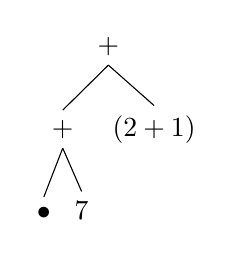
\begin{tikzpicture}
      \Tree [.\(+\) [.\(+\) [.\(\bullet\) ]
                    [.\(7\) ]]
                [.\((2+1)\) ] ]
    \end{tikzpicture}
  \end{center}

  Here are some more examples:
  \begin{center}
    \begin{tabular}{c c c}
      \toprule
      Expression & Context & Redex \\ \midrule
      \((\plambda{x \of \pint}{x + 1})(1+1)\) &
        \((\plambda{x \of \pint}{x + 1}) \bullet\) &
        \(1 + 1\) \\
      \((\plambda{x \of \pint}{x + 1})2\) &
        \(\bullet\) &
        \((\plambda{x \of \pint}{x + 1})2\) \\
      \(2 + 1\) &
        \(\bullet\) &
        \(2 + 1\) \\
      \bottomrule
    \end{tabular}
  \end{center}
\end{example}
For any expression, we can decompose it into a context and a redex.
Then, apply the reduction rule to the redex and repeat.

\subsection{Preservation}
When we used big-step semantics, we can prove global preservation.
In particular, we can prove this by induction on the structure of derivation
of \(e_1 \to e_2\).

\begin{adhoctheorem}{Recall}
  To prove \(Q(e) \implies P(e)\) by induction on the structure of derivation,
  \begin{enumerate}[nosep]
    \item Prove the base cases, i.e.\ prove \(P(e)\) holds for any \(e\)
          in which the proof tree for \(Q(e)\) has depth \(1\).
    \item Prove the inductive step, i.e.\ prove \(P(e)\) holds for any \(e\)
          in which the proof tree for \(Q(e)\) has height \(h+1\),
          assuming that \(P(e')\) holds for any \(e'\)
          in which the proof tree of \(Q(e')\) has height \(h\).
  \end{enumerate}
\end{adhoctheorem}

\begin{proposition}[Global preservation]
  \(e_1 \to e_2 \implies \Gamma \vdash e_1 \of \tau
                \implies \Gamma \vdash e_2 \of \tau\).
\end{proposition}
\begin{proof}
  We proceed by induction on \(e_2\).
  Here \(Q(e_1, e_2) = (e_1 \to e_2)\) and
  \(P(e_1, e_2) = (\Gamma \vdash e_1 \of \tau
                   \implies \Gamma \vdash e_2 \of \tau)\).

  \paragraph{Base cases}
  There are two base cases corresponding to
  \[
    \prfaxiom{x \to x} \qquad
    \prfaxiom{\lambda x. e \to \lambda x. e}
  \]
  In particular,
  \begin{gather*}
    \Gamma \vdash x \of \tau \implies \Gamma \vdash x \of \tau \\
    \Gamma \vdash \lambda x.e \of \tau
      \implies \Gamma \vdash \lambda x.e \of \tau
  \end{gather*}
  are both true.

  \paragraph{Inductive case}
  We have the operational rule
  \[
    \prftree{e_1 \to \lambda x. e_1'}
            {e_1'[e_2 / x] \to e_3}
            {e_1 e_2 \to e_3}
  \]
  We want to prove
  \[
    \Gamma \vdash e_1 e_2 \of \tau \implies \Gamma \vdash e_3 \of \tau,
  \]
  given the induction hypotheses
  \begin{gather}
    \forall t. (\Gamma \vdash e_1 \of t
      \implies \Gamma \vdash \lambda x. e_1' \of t) \label{preservation-1} \\
    \forall t. (\Gamma \vdash e_1'[e_2/x] \of t
      \implies \Gamma \vdash e_3 \of t). \label{preservation-2}
  \end{gather}
  
  From the typing rule
  \[
    \prftree{\Gamma \vdash e_1 \of \tau' \to \tau}
            {\Gamma \vdash e_2 \of \tau'}
            {\Gamma \vdash e_1 e_2 \of \tau}
  \]
  so we know there exists some \(\tau'\)
  such that \(\Gamma \vdash e_1 \of \tau' \to \tau\) and
  \(\Gamma \vdash e_2 \of \tau'\).
  By \cref{preservation-1},
  we have \(\Gamma \vdash \lambda x.e_1' \of \tau' \to \tau\).
  From the typing rule
  \[
    \prftree{\Gamma, x \of \tau' \vdash e_1' \of \tau}
            {\Gamma \vdash (\lambda x \of \tau' .\, e_1') \of \tau' \to \tau}
  \]
  we know that \(\Gamma, x \of t' \vdash e_1' \of \tau\).

  We use the following lemma:
  \begin{lemma}
    \[
      \Gamma, x \of \tau' \vdash e_1' \of \tau
        \land \Gamma \vdash e_2 \of \tau'
        \implies \Gamma \vdash e_1'[e_2 / x] \of \tau.
    \]
  \end{lemma}
  The proof is omitted as an exercise.
  The lemma yields \(\Gamma \vdash e_1'[e_2 / x] \of \tau\),
  and from \cref{preservation-2}, we have \(\Gamma \vdash e_3 \of \tau\).
\end{proof}


\subsection{Progress}
\begin{proposition}[Progress]
  If \(\vdash e \of \tau\) and \(e\) is not a value,
  then there exists \(e'\) such that \(e \to e'\)
  (equivalently, there exists \(H\) and \(r\) such that \(e = H[r]\)).

\end{proposition}
To prove progress, we want to use small step semantics,
because we want to talk about steps of evaluation.

\begin{proof}
  We prove this by induction on the derivation of \(\vdash e \of \tau\).
  
  \paragraph{Base cases:}
  We have the base cases
  \[
    \prfaxiom{\Gamma \vdash \ptrue \of \pbool} \qquad
    \prfaxiom{\Gamma \vdash \pfalse \of \pbool} \qquad
    \prfaxiom{\Gamma \vdash N \of \pint} \qquad
    \prftree{x \of \tau \in \Gamma}
            {\Gamma \vdash x \of \tau} \qquad
    \prftree{\Gamma, x \of \tau_1 \vdash e \of \tau_2}
            {\Gamma \vdash (\lambda x\of \tau_2 . e) \of \tau_1 \to \tau_2}
  \]
  Since these are irreducible values, the condition does not hold,
  so these vacuously satisfy the proposition.

  \paragraph{Inductive cases:}
  We have the inductive cases
  \[
    \prftree{\Gamma \vdash e_1 \of \tau' \to \tau}
            {\Gamma \vdash e_2 \of \tau'}
            {\Gamma \vdash e_1 e_2 \of \tau} \quad
    \prftree{\Gamma \vdash e_1 \of \pint}
            {\Gamma \vdash e_2 \of \pint}
            {\Gamma \vdash e_1 + e_2 \of \pint} \quad
    \prftree{\Gamma \vdash e_1 \of \pint}
            {\Gamma \vdash e_2 \of \pint}
            {\Gamma \vdash e_1 = e_2 \of \pbool} \quad
    \prftree{\Gamma \vdash e \of \pbool}
            {\Gamma \vdash e_t \of \tau}
            {\Gamma \vdash e_f \of \tau}
            {\Gamma \vdash \pifthenelse{e}{e_t}{e_f} \of \tau}
  \]
  We will do the proof for
  \[
    \prftree{\Gamma \vdash e \of \pbool}
            {\Gamma \vdash e_t \of \tau}
            {\Gamma \vdash e_f \of \tau}
            {\Gamma \vdash \pifthenelse{e}{e_t}{e_f} \of \tau}
  \]
  The rest of the cases are similar.
  By the inductive hypothesis,
  \(e\) is either a value or can be decomposed into \(e = H[r]\).

  In the first case, \(e\) is just \(\ptrue\) or \(\pfalse\),
  and the entirety of \(e\) is a redex.

  In the second case, we have the context \(\pifthenelse{H}{e_t}{e_f}\).
\end{proof}

\section{Type inference}
Recall the typing rules of typed lambda calculus:
\begin{adhoctheorem}{Typing Rules of \(F_1\)}
  \begin{gather*}
    \prftree{x \of \tau \in \Gamma}
            {\Gamma \vdash x \of \tau} \qquad
    \prftree{(\Gamma, x \of \tau_1) \vdash e \of \tau_2}
            {\Gamma \vdash (\plambda{x \of \tau_1}{e}) \of \tau_1 \to \tau_2} \qquad
    \prftree{\Gamma \vdash e_1 \of \tau' \to \tau}
            {\Gamma \vdash e_2 \of \tau'}
            {\Gamma \vdash e_1 e_2 \of \tau} \\
    \prfaxiom{\Gamma \vdash N \of \pint} \qquad
    \prftree{\Gamma \vdash e_1 \of \pint}
            {\Gamma \vdash e_2 \of \pint}
            {\Gamma \vdash e_1 + e_2 \of \pint} \qquad
    \prftree{\Gamma \vdash e_1 \of \pint}
            {\Gamma \vdash e_2 \of \pint}
            {\Gamma \vdash e_1 = e_2 \of \pbool} \qquad
    \prftree{\Gamma \vdash e \of \pbool}
            {\Gamma \vdash e_t \of \tau}
            {\Gamma \vdash e_f \of \tau}
            {\Gamma \vdash \pifthenelse{e}{e_t}{e_f} \of \tau}
  \end{gather*}
\end{adhoctheorem}

\begin{example}
  Consider whether the expression
  \((\plambda{f \of \pint \to \pint}{f 5})(\plambda{x \of \pint}{x + 1})\)
  is well typed in \(F_1\).
  
  We can construct the following type checking tree from the bottom:
  \[
    \prftree
      {\prftree[r]{\footnotesize(A)}
         {\prftree
            {\prftree[r]{\footnotesize(B)}
               {f \of \pint \to \pint \in f \of \pint \to \pint}
               {f \of \pint \to \pint \vdash f \of \pint \to \tau}
            }
            {\prfaxiom{f \of \pint \to \pint \vdash 5 \of \pint}}
            {f \of \pint \to \pint \vdash f 5 \of \tau}
         }
         {\vdash (\plambda{f \of \pint \to \pint}{f 5}) \of \tau_1 \to \tau}
      }
      {\prftree
         {\prftree
            {\prftree
               {x \of \pint \in x \of \pint}
               {x \of \pint \vdash x \of \pint}
            }
            {\prfaxiom{x \of \pint \vdash 1 \of \pint}}
            {x \of \pint \vdash x + 1 \of \pint}}
         {\vdash (\plambda{x \of \pint}{x + 1}) \of \tau_1 = \pint \to \pint}
      }
      {\vdash (\plambda{f \of \pint \to \pint}{f 5})
              (\plambda{x \of \pint}{x + 1}) \of \tau}
  \]
  At (A), we know that \(\tau_1 = \pint \to \pint\).
  At (B), we know that \(\tau = \pint\),
  so the entire expression is of type \(\pint\).
  The rest of the tree typechecks, so this is well typed.
\end{example}

Note that even if we don't have the type annotations,
we can still have done the same type derivation:
\begin{example}<type-inference>
  We can check the well typed-ness of
  \((\plambda{f}{f 5})(\plambda{x}{x+1})\) in \(F_1\):
  \[
    \prftree
      {\prftree
         {\prftree
            {\prftree[r]{\footnotesize(D)}
               {f \of \tau_4 \to \tau \in f \of \tau_1}
               {f \of \tau_1 \vdash f \of \tau_4 \to \tau}
            }
            {\prfaxiom{f \of \tau_1 \vdash 5 \of \pint}}
            {f \of \tau_1 \vdash f 5 \of \tau}
         }
         {\vdash (\plambda{f}{f 5}) \of \tau_1 \to \tau}
      }
      {\prftree[r]{\footnotesize(A)}
         {\prftree[r]{\footnotesize(B)}
            {\prftree[r]{\footnotesize(C)}
               {x \of \pint \in x \of \tau_2}
               {x \of \tau_2 \vdash x \of \pint}
            }
            {\prfaxiom{x \of \tau_2 \vdash 1 \of \pint}}
            {x \of \tau_2 \vdash x + 1 \of \tau_3}}
         {\vdash (\plambda{x}{x + 1}) \of \tau_1}
      }
      {\vdash (\plambda{f}{f 5})
              (\plambda{x}{x + 1}) \of \tau}
  \]
  \begin{itemize}
    \item From (A), we have \(\tau_1 = \tau_2 \to \tau_3\).
    \item From (B), we have \(\tau_3 = \pint\).
    \item From (C), we have \(\tau_2 = \pint\).
    \item From (D), we have \(\tau_1 = \tau_4 \to \tau\).
  \end{itemize}
  This gives \(\tau_1 = \pint \to \pint\), and
  \(\tau_2 = \tau_3 = \tau_4 = \tau = \pint\).
\end{example}

This is the idea behind type inference:
we can find the types of expressions even if
the types are not explicitly given in the program.
More explicitly, the strategy we used for type inference is
\begin{enumerate}[nosep]
  \item Use the typing rules to find constraints on
        the types of each subexpression.
  \item Solve the resulting system of constraints.
\end{enumerate}

\begin{example}
  To do type inference in Haskell, we do a similar process.
  Suppose we have the function \mintinline{haskell}{twice f x = f (f x)}.
  We can find the most general type for \mintinline{haskell}{twice}
  by doing the following:
  \begin{enumerate}
    \item Assign types to every subexpression:
          \[
            \text{
              \mintinline{text}{x :: t0} \qquad % chktex 26
              \mintinline{text}{f :: t1} \qquad % chktex 26
              \mintinline{text}{f x :: t2} \qquad % chktex 26
              \mintinline{text}{f (f x) :: t3} % chktex 26
            }
          \]
          This implies \mintinline{haskell}{twice :: t1 -> t0 -> t3}. % chktex 26

    \item Set up constraints.
          In this case, we have
          \begin{align*}
            \text{\mintinline{text}{t1 = t0 -> t2}} &\qquad
              \text{from \mintinline{text}{f x}} \\[-1ex]
            \text{\mintinline{text}{t1 = t2 -> t3}} &\qquad
              \text{from \mintinline{text}{f (f x)}}
          \end{align*}
  
    \item Resolve the constraints.
          We have \mintinline{text}{t0 -> t2 = t2 -> t3},
          so \mintinline{text}{t0 = t2} and \mintinline{text}{t2 = t3}.
          This gives \mintinline{haskell}{twice :: (t0 -> t0) -> t0 -> t0}. % chktex 26
  \end{enumerate}
\end{example}



\end{document}

\documentclass[class=scrartcl]{standalone}
\usepackage{chez}

\begin{document}
\begin{question}
  How do we formalize this process?
\end{question}

\subsection{Constraints}
First, we will formalize what a contraint actually is,
talk about how to generate them.

Consider the language of constraints:
\[
  C := \tau_1 = \tau_2 \mid C \lor C
                       \mid \exists \tau. C
\]
We can build constraints from the typing rules
as we build the type checking tree.
The base cases are
\[
  \bbrackets{\Gamma \vdash x \of \tau} = (\Gamma(x) = \tau) \qquad
  \bbrackets{\Gamma \vdash N \of \tau} = (\pint = \tau).
\]
The inductive cases are
\begin{gather*}
  \bbrackets{\Gamma \vdash e_1 e_2 \of \tau}
    = \exists a (\bbrackets{\Gamma \vdash e_1 \of a \to \tau} \land
                 \bbrackets{\Gamma \vdash e_2 \of a}) \\
  \bbrackets{\Gamma \vdash \lambda x. e \of \tau}
    = \exists a_1 a_2. (\bbrackets{\Gamma, x \of a_1 \vdash e \of a_2} \land
                         \tau = a_1 \to a_2) \\
  \bbrackets{\Gamma \vdash e_1 + e_2 \of \tau}
    = \exists a_1 a_2. (\bbrackets{\Gamma \vdash e_1 \of \pint} \land
                        \bbrackets{\Gamma \vdash e_2 \of \pint} \land
                        \tau = \pint)
\end{gather*}

\begin{example}
  Suppose we want to determine the type of
  \[
    \lambda x. x + 1.
  \]
  We can recursively evaluate the type judgement
  \begin{align*}
    \bbrackets{\Gamma \vdash (\plambda{x}{x+1}) 2 \of \tau}
      &= \exists a_1.\,
        \textcolor{chezblue}{
          \bbrackets{\Gamma \vdash (\plambda{x}{x+1}) \of a_1 \to \tau}} \land
        \textcolor{chezgreen}{\bbrackets{\Gamma \vdash 2 \of a_1}} \\
      &= \exists a_1.\,
        \textcolor{chezblue}{(\exists a_2 a_3.\,
          \textcolor{chezpurple}{
            \bbrackets{\Gamma, x \of a_2 \vdash x + 1 \of a_3}} \land
          (a_1 \to \tau = a_2 \to a_3)
        )} \land
        \textcolor{chezgreen}{(a_1 = \pint)} \\
      &= \exists a_1.\,
        \textcolor{chezblue}{(\exists a_2 a_3.\,
          \textcolor{chezpurple}{
            \bbrackets{\Gamma, x \of a_2 \vdash x \of \pint} \land
            \bbrackets{\Gamma, x \of a_2 \vdash 1 \of \pint} \land
            (a_3 = \pint)
          } \land
          (a_1 \to \tau = a_2 \to a_3)
        )} \land
        \textcolor{chezgreen}{(a_1 = \pint)} \\
      &= \exists a_1.\,
        \textcolor{chezblue}{(\exists a_2 a_3.\,
          \textcolor{chezpurple}{
            (a_2 = \pint) \land
            (\pint = \pint) \land
            (a_3 = \pint)
          } \land
          (a_1 \to \tau = a_2 \to a_3)
        )} \land
        \textcolor{chezgreen}{(a_1 = \pint)}.
  \end{align*}
  and this gives us an expression in the language of constraints.
\end{example}

Now that we have constraints,
we want to determine if they are equal, and
whether they can be satisfied with
an appropriate choice of type variables.

To answer the first question,
to determine when two types \(\tau_a\) and \(\tau_b\) are equal,
we use \vocab{structural equality}.
In particular, \(\tau_a = \tau_b\) when their constructors are the same,
and their contents are the same.
For instance, if \(\tau_a = \tau_1 \to \tau_2\) and
                 \(\tau_b = \tau_3 \to \tau_4\),
then \(\tau_a = \tau_b \iff \tau_1 = \tau_3 \land \tau_2 = \tau_4\).

\subsection{Unification}
The answer to the question of how to solve constraints is more complicated.
We define \vocab{unification} to be the process of determining
whether two types can be made equal by selecting appropriate
substitutions for type variables.

First we will formally define types and type substitution.
The language of \vocab{types} is
\begin{alignat*}{4}
  \tau :={} & \iota && \qquad
    \text{base types
          (\mintinline{haskell}{Int}, \mintinline{haskell}{Bool}, \dots)} \\
  \mid{} & t && \qquad\text{type variables} \\
  \mid{} & \tau_1 \to \tau_2 && \qquad\text{function types}.
\end{alignat*}
A \vocab{type substitution} is a map
\begin{align*}
  S \colon& \set{\text{type variables}} \to \set{\text{types}} \\[-1ex]
  S ={}& [\tau_1/t_1, \tau_2/t_2, \dots, \tau_n/t_n],
\end{align*}
and when \(\tau' = S \tau\),
we say \(\tau'\) is a \vocab{substitution instance} of \(\tau\).

\begin{example}
  If we have \(S_1 = [(t \to \pbool) / t_1]\) and \(S_2 = [\pint / t]\), then
  \begin{align*}
    S_2 S_1 (t_1 \to t_1) &= S_2 ((t \to \pbool) \to (t \to \pbool)) \\
      &= (\pint \to \pbool) \to (\pint \to \pbool).
  \end{align*}
\end{example}

To determine whether two types are able to be unified,
we use the following algorithm:
\begin{minted}[escapeinside=||]{haskell}
unify(|\(\tau_1\)|, |\(\tau_2\)|) =
  case (|\(\tau_1\)|, |\(\tau_2\)|) of
    |\((\tau_1, t_2\))| -> |\([\tau_1/t_2]\)| given |\(t_2 \notin FV(\tau_1)\)|
    |\((t_1, \tau_2\))| -> |\([\tau_2/t_1]\)| given |\(t_1 \notin FV(\tau_2)\)|
    |\((\iota_1, \iota_2\))| -> if (eq |\(\iota_1\)| |\(\iota_2\)|) then []
                          else Fail
    |\((\tau_{11} \to \tau_{12}, \tau_{21} \to \tau_{22}\))| -> let |\(S_1 = {}\)|unify|\((\tau_{11}, \tau_{21})\)|
                              |\(S_2 = {}\)|unify|\((S_1 \tau_{12}, S_1 \tau_{22})\)|
                          in |\(S_2 S_1\)|
    otherwise -> Fail
\end{minted}

\subsection{Putting it together}
Now that we have formalized both constraints and unification,
we can combine them into a type inference algorithm.
In the examples above (e.g.\ \cref{ex:type-inference}),
we collected all of the constraints,
and then at the end we solved the system.
However in practice, this can be inefficient if your program is large,
so we often solve the constraints incrementally,
and build the substitution map incrementally.

Let us come up with an inference algorithm \(W\) such that
\(W(\textrm{TE}, e) = (S, \tau)\), where \(S(\textrm{TE}) \vdash e \of \tau\).
Here, we are writing \(\textrm{TE}\) instead of \(\Gamma\) for convenience.
Intuitively, the type environment \(\textrm{TE}\) stores
  the most general type of each identifier while
the substitution \(S\) stores the changes in type variables.

Naturally, we will do casework on \(e\). We have
\begin{gather*}
  \bbrackets{\Gamma \vdash N \of \tau} = (\pint = \tau) \qquad
    \bbrackets{\Gamma \vdash x \of \tau} = (\Gamma(x) = \tau) \\
  \bbrackets{\Gamma \vdash e_1 e_2 \of \tau}
    = \exists a (\bbrackets{\Gamma \vdash e_1 \of a \to \tau} \land
                 \bbrackets{\Gamma \vdash e_2 \of a}) \\
  \bbrackets{\Gamma \vdash \lambda x. e \of \tau}
    = \exists a_1 a_2. (\bbrackets{\Gamma, x \of a_1 \vdash e \of a_2} \land
                         \tau = a_1 \to a_2).
\end{gather*}
This gives us the algorithm
\begin{minted}[escapeinside=||]{haskell}
w(te, e) = case e of
  c    -> ({}, Int)
  x    -> if (x |\(\in\)| te) then ({}, te[x])
                      else Fail
  |\(\lambda\)|x.e -> let (|\(S_1\)|, |\(\tau_1\)|) = w(te |\(\union\)| {x:u}, e)
           in (|\(S_1\)|, |\(S_1\)|(u) -> |\(\tau_1\)|)
  |\(e_1 e_2\)|  -> let (|\(S_1\)|, |\(\tau_1\)|) = w(te, |\(e_1\)|)
              (|\(S_2\)|, |\(\tau_2\)|) = w(|\(S_1\)|(te), |\(e_2\)|)
              |\(S_3\)| = unify(|\(S_2\)|(|\(\tau_1\)|), |\(\tau_2\)| -> u)
           in (|\(S_3 S_2 S_1\)|, |\(S_3\)|(u))
\end{minted}

\begin{example}
  We can even run this algorithm by hand:
  Let's say we are trying to compute
  \(W(\nullset, (\plambda{f}{f 5})(\plambda{x}{x}))\).
  \begin{adhoctheorem*}{Computation}[Application]
    Let \((S_1, \tau_1) = W(\nullset, \plambda{f}{f 5})
                        = (S_1', S_1'(u_1) \to \tau_1')
                        = ([\pint \to u_2 / u_1], (\pint \to u_2) \to u_2)\),
    with subvariables obtained from the following subcomputation:
    \begin{adhoctheorem*}{Computation}[Lambda]
      Let \((S_1', \tau_1') = W(\nullset \union \set{f \of u_1}, f 5)
                            = (S_3'' S_2'' S_1'', S_3'' u_2)
                            = ([\pint \to u_2 / u_1], u_2)\)
      with subvariables obtained from the subcomputation:
      \begin{adhoctheorem*}{Computation}[Application]
        Let \((S_1'', \tau_1'') = W(\set{f \of u_1}, f) = (\nullset, u_1)\).

        Let \((S_2'', \tau_2'') = W(\set{f \of u_1}, 5) = (\nullset, \pint)\).

        Let \(\begin{aligned}[t]
            S_3'' &= \pname{unify}(S_2''(u_1), \pint \to u_2) \\[-1ex]
                  &= \pname{unify}(u_1, \pint \to u_2) \\[-1ex]
                  &= [\pint \to u_2 / u_1]
          \end{aligned}\).
      \end{adhoctheorem*}
    \end{adhoctheorem*}

    Let \((S_2, \tau_2) = W(S_1' \nullset, \plambda{x}{x})
                        = (S_1', S_1'(u_3) \to \tau_1')
                        = (\nullset, u_3 \to u_3)\),
    with subvariables obtained from the subcomputation:
    \begin{adhoctheorem*}{Computation}[Lambda]
      Let \((S_1', \tau_1') = W(\nullset \union \set{x \of u_3}, x)
                            = (\nullset, u_3).\)
    \end{adhoctheorem*}

    Let \(S_3 = \pname{unify}(S_2(\tau_1), \tau_2 \to u_4)
              = \pname{unify}((\pint \to u_2) \to u_2, (u_3 \to u_3) \to u_4)
              = S_2' S_1'
              = [ \pint / u_2
                , \pint / u_3
                , \pint / u_4
                ]\),
    with subvariables obtained from the subcomputation:
    \begin{adhoctheorem*}{Computation}[Unify]
      Let \(S_1' = \pname{unify}(\pint \to u_2, u_3 \to u_3)
                 = S_2'' S_1''
                 = [ \pint / u_2
                   , \pint / u_3
                   ]\),
      with subvariables obtained from:
      \begin{adhoctheorem*}{Computation}[Unify]
        Let \(S_1'' = \pname{unify}(\pint, u_3)
                    = [\pint / u_3]\).

        Let \(S_2'' = \pname{unify}(S_1'' u_2, S_1'' u_3)
                    = \pname{unify}(u_2, \pint)
                    = [\pint / u_2]\).
      \end{adhoctheorem*}

      Let \(S_2' = \pname{unify}(S_1' u_2, S_1' u_4)
                 = \pname{unify}(\pint, u_4)
                 = [\pint / u_4]\)
    \end{adhoctheorem*}
  \end{adhoctheorem*}
  
  This gives \(W(\nullset, (\plambda{f}{f 5})(\plambda{x}{x}))
                 = (S_3 S_2 S_1, S_3 u_4)
                 = ([ \pint / u_1
                    , \pint / u_2
                    , \pint / u_3
                    , \pint / u_4
                    ], \pint)\).
\end{example}

We can include the \(\pletin{\dots}{\dots}\) construct with the typing rule
\[
  \prftree{\Gamma, x \of \tau' \vdash e_1 \of \tau'}
          {\Gamma, x \of \tau' \vdash e_2 \of \tau}
          {\Gamma \vdash \pletin{x = e_1}{e_2} \of \tau}
\]
This gives the constraint rule
\[
  \bbrackets{\Gamma \vdash \pletin{x = e_1}{e_2} \of \tau}
    = \exists \tau'. \bbrackets{\Gamma, x \of \tau' \vdash e_1 \of \tau'} \land
                     \bbrackets{\Gamma, x \of \tau' \vdash e_2 \of \tau}.
\]
This gives the type inference case:
\begin{minted}[escapeinside=||]{haskell}
w(te, e) = case e of
  (let |\(x = e_1\)| in |\(e_2\)|) -> let (|\(S_1\)|, |\(\tau_1\)|) = w(te |\(\union\)| {x:u}, |\(e_1\)|)
                           |\(\,S_2\)|      = unify (|\(S_1\)(u)|, |\(\tau_1\)|)
                           (|\(S_3\)|, |\(\tau_2\)|) = w(|\(S_2\)||\(S_1\)|(te) |\(\union\)| {x:|\(\tau_1\)|}, |\(e_2\)|)
                        in (|\(S_3 S_2 S_1\)|, |\(\tau_2\)|)
\end{minted}








\end{document}

\documentclass[class=scrartcl]{standalone}
\usepackage{chez}

\begin{document}

\section{Polymorphism}
Under our current rules,
\(\pletin{\pname{id} = \plambda{x}{x}}
         {(\dots (\pname{id} \ptrue) \dots (\pname{id} 1) \dots)}\)
is not well typed, because \(\pname{id}\) cannot be both
\(\pint \to \pint\) and \(\pbool \to \pbool\).
There are a few ways we can try to fix this:
\begin{description}
  \item [Explicit polymorphism] We introduce a type-level lambda expression,
        formalized with the typing rules
        \[
          \prftree{\Gamma \vdash e \of \tau}
                  {\Gamma \vdash \Lambda t.\, e
                                 \of \forall t. \tau} \qquad
          \prftree{\Gamma \vdash e \of \forall t. \tau'}
                  {\Gamma \vdash e[\tau] \of \tau'[\tau / t]}
        \]
        For instance, we have \(\pname{id} = \Lambda T \operatorname{.}
                                                     \plambda{x \of T}{x}\),
        and when we want to use it, we write \(\pname{id}[\pint]5\).
        However, this is annoying because we have to explicitly
        pass in the type whenever we use it.
  \item [Impredicative polymorphism] We allow self referential types,
        formalized by the language of types and expressions:
        \begin{align*}
          \tau &\coloneqq b \mid \tau_1 \to \tau_2
                            \mid T
                            \mid \forall T. \tau \\
          e    &\coloneqq x \mid \plambda{x \of \tau}{e}
                            \mid e_1 e_2
                            \mid \Lambda T.\, e
                            \mid e[\tau]
        \end{align*}
        Note that here, we can define
        a type variable \(t = \forall x. x \to x\),
        where \(x\) can refer to \(t\).
        This is powerful, but we cannot express recursion.
        Moreover, type inference is undecidable.
  \item [Predicative polymorphism] We restrict impredicativity to get
        the language of types and expressions:
        \begin{align*}
          \tau   &\coloneqq b \mid \tau_1 \to \tau_2
                              \mid T \\
          \sigma &\coloneqq \tau \mid \forall T .\, \tau
                                 \mid \sigma_1 \to \sigma_2 \\
          e      &\coloneqq x \mid \lambda\, x \of \sigma .\, e
                              \mid e_1 e_2
                              \mid \Lambda T .\, e
                              \mid e[\tau]
        \end{align*}
        This is still very powerful,
        but we cannot instantiate a polymorphic type.
        Moreover, type inference is still undecidable.
  \item [Prenex predicative polymorphism] We restrict so that
        all quantifiers are at the beginning.
        This gives us the grammar
        \begin{align*}
          \tau   &\coloneqq b \mid \tau_1 \to \tau_2
                              \mid T \\
          \sigma &\coloneqq \tau \mid \forall T .\, \tau \\
          e      &\coloneqq x \mid \lambda\, x \of \tau .\, e
                              \mid e_1 e_2
                              \mid \Lambda T .\, e
                              \mid e[\tau]
        \end{align*}
        This makes our type inference decidable,
        but now we cannot pass polymorphic functions as function arguments.
\end{description}
The compromise we will settle on is called let polymorphism.
In particular, we introduce the expression type of the form
\(\pletin{x = e_1}{e_2}\), which is equivalent to
\((\plambda{x}{e_2}){e_1}\), except \(x\) can be polymorphic.
This gives a good amount of expressiveness,
while maintaining decidability.
This is called the Hindley-Milner type system.


\section{Type inference with polymorphism}
If we have
\(\pletin{(\pname{id} = \lambda x. x)}
         {\dots (\pname{id} 1) \dots (\pname{id} \ptrue) \dots}\),
we can come up with multiple constraints
\[
  \pname{id} \of t_1 \to t_1 \qquad
  \pname{id} \of \pint \to t_1 \qquad
  \pname{id} \of \pbool \to t_1,
\]
which do not unify.
The solution to this is to generalize the type to
\[
  \pname{id} \of \forall t_1.\, t_1 \to t_1.
\]
Then, we can instantiate the generalized type variable
differently in different contexts.
\[
  \pname{id}_1 \of \pint \to \pint \qquad
  \pname{id}_2 \of \pbool \to \pbool,
\]

\subsection{Hindley-Milner types}
Consider the language
\begin{align*}
  E \coloneqq{} & c                     && \text{constant} \\[-1ex]
    {}\mid{}    & x                     && \text{variable} \\[-1ex]
    {}\mid{}    & \lambda x. E          && \text{abstraction} \\[-1ex]
    {}\mid{}    & (E_1 E_2)             && \text{application} \\[-1ex]
    {}\mid{}    & \pletin{x = E_1}{E_2} && \text{let-block}
\end{align*}
Note that there are no explicit types in the language!
All types are inferred according to the
\vocab{Hindley-Milner type inference algorithm}.

The types are
\begin{align*}
  \tau \coloneqq{} & \iota             && \text{base types} \\[-1ex]
       {}\mid{}    & t                 && \text{type variables} \\[-1ex]
       {}\mid{}    & \tau_1 \to \tau_2 && \text{function types},
\end{align*}
and there are type schemes
\[
  \sigma := \tau \mid \forall t.\, \sigma.
\]
Note that all of the \(\forall\)s occur at the beginning of a type scheme,
so a type \(\tau\) cannot contain a type scheme \(\sigma\).

A \vocab{type environment} is a mapping from identifiers to type schemes.

A type scheme \(\sigma = \forall t_1 \dots t_n.\, \tau\)
can be \vocab{instantiated} into a type \(\tau'\) by
substituting types for the bound variables \(t_1, \dots, t_n\) of \(\sigma\),
i.e.\ \(\tau' = S \tau\) for some substitution \(S\) with
\(\operatorname{Dom}(S) \subseteq \operatorname{BV}(\sigma)\).
We then say that \(\tau'\) is an \vocab{instance} of \(\sigma\),
and write \(\sigma > \tau'\).
We call \(\tau'\) a \vocab{generic instance} of \(\sigma\) if \(S\) maps
\(t_1, \dots, t_n\) to new type variables.

\begin{example}
  If we have \(\sigma = \forall t_1.\, t_1 \to t_1\), then
  \begin{itemize}[nosep]
    \item \(t_3 \to t_2\) is a generic instance of \(\sigma\), and
    \item \(\pint \to t_2\) is a non-generic instance of \(\sigma\).
  \end{itemize}
\end{example}

We can go in the other direction.
In particular, we can generalize types with free variables:
\[
  \operatorname{Gen}(\mathrm{TE}, \tau)
    = \forall t_1 \dots t_n.\, \tau
  \qquad \text{where} \qquad
  \set{t_1, \dots, t_n}
    = \operatorname{FV}(\tau) \setminus \operatorname{FV}(\mathrm{TE}).
\]
This captures the notion of \emph{new} type variables in \(\tau\),
and introduces polymorphism.
In particular, we quantify the type variables that are free in \(\tau\)
but not in the type environment \(\mathrm{TE}\).

Overall, this gives us the type inference rules:
\begin{gather*}
  \prftree[r]{\footnotesize (App)}
          {\Gamma \vdash e_1 \of \tau \to \tau'}
          {\Gamma \vdash e_2 \of \tau}
          {\Gamma \vdash (e_1 e_2) \of \tau'} \qquad
  \prftree[r]{\footnotesize (Abs)}
          {\Gamma \vdash e_1 \of \tau \to \tau'}
          {\Gamma \vdash e_2 \of \tau}
          {\Gamma \vdash (e_1 e_2) \of \tau'} \qquad
  \prftree[r]{\footnotesize (Var)}
          {x \of \sigma \in \Gamma}
          {\sigma \geq \tau}
          {\Gamma \vdash x \of \tau} \\
  \prftree[r]{\footnotesize (Const)}
          {\operatorname{typeof}(c) \geq \tau}
          {\Gamma \vdash c \of \tau} \qquad
  \prftree[r]{\footnotesize (Let)}
          {\Gamma; \braces{x \of \tau} \vdash e_1 \of \tau}
          {\Gamma; \braces{x \of \operatorname{Gen}(\Gamma, \tau)}
            \vdash e_2 \of \tau'}
          {\Gamma \vdash (\pletin{x = e_1}{e_2}) \of \tau'}
\end{gather*}

The important rules for polymorphism is in (Var) and (Let).
In particular, the type of a variable is generalized in the let expression,
and then the type scheme can be specialize to different types with the Var rule.

\subsection{HM Inference algorithm}
Our type inference algorithm changes a bit to account for polymorphism,
and we get the following:
\begin{minted}[escapeinside=||]{haskell}
w (te, e) = case e of
  c    -> ({}, typeof(c))
  x    -> if (x |\(\notin\)| te) then Fail
                      else let |\(\forall t_1 \dots t_n.\, \tau\)| = TE[x]
                            in ({}, |\([u_i / t_i] \tau\)|)
  |\(\lambda\)|x.e -> let (|\(S_1\)|, |\(\tau_1\)|) = w(te |\(\union\)| {x:u}, e)
           in (|\(S_1\)|, |\(S_1\)|(u) -> |\(\tau_1\)|)
  |\(e_1 e_2\)|  -> let (|\(S_1\)|, |\(\tau_1\)|) = w(te, |\(e_1\)|)
              (|\(S_2\)|, |\(\tau_2\)|) = w(|\(S_1\)|(te), |\(e_2\)|)
              |\(S_3\)| = unify (|\(S_2\)|(|\(\tau_1\)|), |\(\tau_2\)| -> u)
           in (|\(S_3 S_2 S_1\)|, |\(S_3\)|(u))
  (let |\(x = e_1\)| in |\(e_2\)|) -> let (|\(S_1\)|, |\(\tau_1\)|) = w(te |\(\union\)| {x:u}, |\(e_1\)|)
                           |\(\,S_2\)|      = unify(|\(S_1\)(u)|, |\(\tau_1\)|)
                           |\(\,\sigma\)|       = gen(|\(S_2 S_1\)(TE)|, |\(S_2(\tau_1)\)|)
                           (|\(S_3\)|, |\(\tau_2\)|) = w(|\(S_2\)||\(S_1\)|(te) |\(\union\)| {x:|\(\sigma\)|}, |\(e_2\)|)
                        in (|\(S_3 S_2 S_1\)|, |\(\tau_2\)|)
\end{minted}

The only differences are in the variable case and the let case,
where we specialize and generalize respectively.

Some important observations about HM type inference:
\begin{itemize}[nosep]
  \item We do not generalize type variables that are used elsewhere.
  \item Let is the only way of defining polymorphic constructs.
  \item We generalize the types of the let bindings
        \emph{after} processing their definitions.
\end{itemize}

HM type inference is sound and generates the most general types of expressions.
Therefore, an inferred type is verifiable and any verifiable type is inferred.
This complexity of HM type inference is \textsf{PSPACE}-hard,
due to the nested let blocks.

\begin{example}
  Consider
  \begin{minted}[linenos=false]{haskell}
let twice f x = f (f x)
 in twice twice succ 4
  \end{minted}
  and
  \begin{minted}[linenos=false]{haskell}
let twice f x = f (f x)
    foo g = (g g succ) 4
 in foo twice
  \end{minted}
  In the first example, \mintinline{haskell}{twice} has a generic type,
  while in the second example, \mintinline{haskell}{g} has a non-generic type.
  This means that \mintinline{haskell}{foo} in
  the second example is not type correct.
\end{example}

Some extensions that we can think about are:
\begin{description}[nosep]
  \item [Type declarations] for sanity checks, and for relaxed restrictions.
  \item [Incremental type checking] if the whole program is not given at
        the same time, we can still soundly infer the types.
  \item [Typing references to mutable objects] HM is unsound
        for a language with refs (mutable locations).
  \item [Overloading resolution]
\end{description}









\end{document}

\documentclass[class=scrartcl]{standalone}
\usepackage{chez}

\begin{document}
\subsection{Type classes}
Hindley-Milner gives us generic functions that
make no assumptions about the type, like
\begin{minted}{haskell}
const :: forall a b. a -> b -> a
const x y = x

const :: forall a b. (a -> b) -> a -> b
apply f x = f x
\end{minted}

However, what if we \emph{do} need to make assumptions about the types?
For instance, if we have the list data type (written two ways for clarity):
\begin{minted}{haskell}
data List x = Nil | Cons x (List x)
data [x] = [] | x:[x]
\end{minted}
we can then write a sum function (with an accumulator)
\begin{minted}{haskell}
sum n [] = n
sum n (x:xs) = sum (n + x) xs
\end{minted}
The type of \mintinline{haskell}{sum}
cannot be \texttt{a -> [a] -> a}
because we have a restriction on the type
(namely that we need to be able to add \texttt{a}s).

The solution to this is to pass in the notion of plus:
\begin{minted}{haskell}
sum plus n [] = n
sum plus n (x:xs) = sum (plus n x) xs
\end{minted}
Now we have a polymorphic type for sum
\mintinline{haskell}{sum :: (a -> a -> a) -> a -> [a] -> a} % chktex 26
When we want to call \mintinline{haskell}{sum},
we have to pass in the appropriate function representing addition.

If we want to write other functions like \mintinline{haskell}{sum},
we also need to use arithmetic operations.
We can generalize if we include a set of functions
\(\set{+, -, \times, \obelus}\).
In particular, we can create a ``class'' type:
\begin{minted}{haskell}
data (Num a) = Num {
  (+) :: a -> a -> a
  (-) :: a -> a -> a
  (*) :: a -> a -> a
  (/) :: a -> a -> a
  fromInteger :: Integer -> a
}
\end{minted}
Then we can use this group of functions to represent restrictions on type:
\begin{minted}{haskell}
sum       :: Num a -> a -> [a] -> a
matrixMul :: Num a -> Mat a -> Mat a -> Mat a
dft       :: Num a -> Vec a -> Vec a -> Vec a
\end{minted}
Then, all of the numeric aspects of the type
can be isolated to the \mintinline{haskell}{Num} type.
For each type that has properties of a number,
we can build a \mintinline{haskell}{Num} instance
and functions that need to use properties of a number
will take it as an argument.

We can use the same idea to encompass other ideas,
like equality, ordering, and conversion to/from \mintinline{haskell}{String}.

However, this is slightly annoying when
we have to manually pass in \mintinline{haskell}{Num} objects.
We have to keep track of the \mintinline{haskell}{Num} objects,
and make sure that our \mintinline{haskell}{Num}
instances are consistent with each other
(e.g.\ \mintinline{haskell}{Num a} and \mintinline{haskell}{Num (Mat a)}
 are related to each other in a reasonable way.)
The way we solve this is we move class objects into a type class.

\begin{definition}
  A \vocab{type class} is a group of related functions
  that are overloaded over types.
\end{definition}

We can define the typeclass
\begin{minted}{haskell}
class Num a where
  (+), (-), (*) :: a -> a -> a
  negate        :: a -> a
  ...
\end{minted}
and then define instances:
\begin{minted}{haskell}
instance Num Int where
  x + y = integer_add x y
  x - y = integer_sub x y
  ...

instance Num Float where
  ...
\end{minted}

We can also define hierarchical data types:
\begin{minted}{haskell}
class Eq a where
  (==), (/=) :: a -> a -> Bool

class (Eq a) => (Ord a) where
  (<), (<=), (>=), (>) :: a -> a -> Bool
  max, min             :: a -> a -> a
\end{minted}
Here, \mintinline{haskell}{Eq} is a superclass of \mintinline{haskell}{Ord},
so every instance of \mintinline{haskell}{Ord} is
also an instance of \mintinline{haskell}{Eq}.

Each type class corresponds to one ``concept'' and class constraints
gives a natural hierarchy on type classes.
Often, a type class has laws that are associated with it.
For instance, in \mintinline{haskell}{Num},
the function \mintinline{haskell}{(+)} should be associative and commutative.
These aren't checked by the compiler, so the programmer has to ensure that
every instance follows these laws.

If we view type classes as predicates,
the type checked can deal with all of the passing
that we had to manually do before.
Note that while this looks like a new feature,
the compiler desugars this into pure \(\lambda\)-calculus.

\subsection{Subtyping}
When working with lambda calculus,
we may notice that it can be annoyingly rigid.
For instance, \((\plambda{r \of \braces{x \of \pint}}{r[x]})\braces{x=0, y=1}\)
seems well-behaved, but is not well typed,
since the argument has type \(\braces{x \of \pint, y \of \pint}\)
while the function accepts type \(\braces{x \of \pint}\).
The goal of subtyping is to refine the typing rules so that
they accept terms like the one above.

If we have some operator \(\bbrackets{\cdot}\) where
\(\bbrackets{\tau}\) represents a set that represents \(\tau\), we have
e.g.\ \(\bbrackets{\pint} = \ZZ\) and \(\bbrackets{\textsf{float}} = \RR\).
Then we may try to define \(\tau_1 \leq \tau_2\) if and only if
\(\bbrackets{\tau_1} \subseteq \bbrackets{\tau_2}\).
A more useful rule is that \(\tau_1 \leq \tau_2\) if,
we can use a \(\tau_1\) everywhere we can use a \(\tau_2\).
For instance, any integer \(N\) can be treated as
a real with no loss of meaning.

The typing rule for this, called \vocab{subsumption}, is
\[
  \prftree{\Gamma \vdash e \of \tau'}
          {\tau' \leq \tau}
          {\Gamma \vdash e \of \tau}
\]

To determine the pairs of subtypes, we can provide a list to the compiler.
However, there is a better way to come up with the subtyping rules
that does not require the user to explicitly declare them.
A \vocab{structural subtyping} system includes rules
that can analyze the structure of types to deduce subtyping rules,
rather than just using the rules that the user explicitly defined.

\subsubsection{Product types}
Consider the product type \(\tau_1 \times \tau_2\).
\[
  \prftree{\tau_1 \leq \tau_1'}
          {\tau_2 \leq \tau_2'}
          {\tau_1 \times \tau_2 \leq \tau_1' \times \tau_2'}
\]
We say that the product type constructor is \vocab{covariant}.

\subsubsection{Record types}
A more general type is a record type
\(\set{a_1 \of \tau_1, \dots, a_N \of \tau_N}\),
where for every \(i\), there is a field \(a_i\) of type \(\tau_i\).

Then there are two types of subtyping:
\[
  \set{a \of \textsf{Int}, b \of \textsf{Alice}}
    \leq \set{a \of \textsf{Number}, b \of \textsf{Person}},
\]
called depth subtyping, and
\[
  \set{a \of \textsf{Number}, b \of \textsf{Person}, c \of \textsf{Tool}}
    \leq \set{a \of \textsf{Number}, b \of \textsf{Person}},
\]
called width subtyping.

We can formalize these into the typing rules:
\[
  \prftree[r]{depth}
          {\forall i. \tau_i \leq \tau_i'}
          {\set{a_i \of \tau_i} \leq \set{a_i \of \tau_i'}}
  \qquad \qquad
  \prftree[r]{width}
          {\forall j. \exists i. a_i = a_j' \land \tau_i \leq \tau_j'}
          {\set{a_i \of \tau_i} \leq \set{a_j \of \tau_j'}}
\]

\subsubsection{Function types}
For function types \(\tau_1 \to \tau_2\),
we could optimistically guess
\[
  \prftree{\tau_1 \leq \tau_1'}
          {\tau_2 \leq \tau_2'}
          {\tau_1 \to \tau_2 \leq \tau_1' \to \tau_2'}
\]
However, we cannot use a \(\pint \to \pint\) anywhere we can use a
\(\textsf{float} \to \pint\), as our subtype function cannot take all
of the inputs that the original function could.
The fix to this is to switch the subtyping direction of the input type.
\[
  \prftree{\tau_1 \geq \tau_1'}
          {\tau_2 \leq \tau_2'}
          {\tau_1 \to \tau_2 \leq \tau_1' \to \tau_2'}
\]
We say that the function type is \vocab{contravariant} in the domain
and covariant in the codomain.

\subsubsection{Array and list types}
For for \emph{mutable} arrays \(\tau[]\),
the operations we can perform on them are
both reading or writing to some entry of the array.
There are two possible options for a typing rule if we were to have one,
a covariant and contravariant rule, which are respectively:
\[
  \prftree{\tau_1 \leq \tau_2}
          {\tau_1[] \leq \tau_2[]} \qquad
  \prftree{\tau_1 \geq \tau_2}
          {\tau_1[] \leq \tau_2[]}
\]
In the covariant case, note that we cannot
write a \(\tau_2\) into a \(\tau_1[]\),
and in the contravariant case, we cannot
read a \(\tau_2\) from a \(\tau_1[]\).
Therefore, arrays cannot be subtyped.
For this reason, we call arrays \vocab{invariant}.

For \emph{immutable} lists \([\tau]\), we have
\[
  \prftree{\tau_1 \geq \tau_2}
          {[\tau_1] \leq [\tau_2]}
\]
In general, most ``data structures'' are covariant.


\section{Monads}
These notes contain a different explanation of monads
than what was presented in lecture.
I personally believe that this explanation is a better introduction.
Explanations inspired by:
\url{https://mightybyte.github.io/monad-challenges/}


\subsection{Maybe monad}
Suppose we have some functions that may fail:
Recall the \mintinline{haskell}{Maybe a} type in Haskell:
\begin{minted}{haskell}
data Maybe a = Nothing | Just a
\end{minted}
Suppose we have the functions
\begin{minted}{haskell}
tailMaybe :: [a] -> Maybe [a]
tailMaybe [] = Nothing
tailMaybe (x:xs) = Just xs

maximumMaybe :: Ord a => [a] -> Maybe a
maximumMaybe [] = Nothing
maximumMaybe xs = Just $ foldl1 max xs

reciprocalMaybe :: (Eq a, Fractional a) => a -> Maybe a
reciprocalMaybe 0 = Nothing
reciprocalMaybe n = Just $ 1/n
\end{minted}
and we want to compose these.
The standard way to do this is
to case match on each result like so:
\begin{minted}{haskell}
f :: (Ord a, Fractional a) => [a] -> Maybe a
f xs =
  case tailMaybe xs of
    Nothing -> Nothing
    Just ys -> case maximumMaybe ys of
                 Nothing -> Nothing
                 Just m  -> reciprocalMaybe m
\end{minted}
However, this gets annoying once we have a lot of functions.
We can abstract over this:
We define a function to facilitate this composition
\begin{minted}{haskell}
bind :: Maybe a -> (a -> Maybe b) -> Maybe b
bind Nothing _ = Nothing
bind (Just a) f = f a
\end{minted}
Then, we can rewrite our function
\begin{minted}{haskell}
f :: (Ord a, Fractional a) => [a] -> Maybe a
f xs = bind (bind (tailMaybe xs) maximumMaybe) reciprocalMaybe
\end{minted}
If we define another function to ``inject''
a value into the \mintinline{haskell}{Maybe} context,
we can use \mintinline{haskell}{bind} with infix notation:
\begin{minted}{haskell}
pure x = Just x   :: a -> Maybe a
(>>=) = bind      :: Maybe a -> (a -> Maybe b) -> Maybe b

f :: (Ord a, Fractional a) => [a] -> Maybe a
f xs = pure xs >>= tailMaybe >>= maximumMaybe >>= reciprocalMaybe
\end{minted}

\subsection{Writer monad}
Suppose we have some functions
\begin{minted}{haskell}
plusOne x = x + 1
square x = x * x
\end{minted}
that we wanted to augment by letting them append to a log.
One idea we may think of is to also return a string that we can look at:
\begin{minted}{haskell}
plusOne' x = (x + 1, "added one")
square' x = (x * x, "squared")
\end{minted}
However, this breaks compositionality, because
\mintinline{haskell}{plusOne' (square' x)}
does not typecheck like
\mintinline{haskell}{plusOne (square x)}
does.
In particular, composition becomes really annoying:
\begin{minted}{haskell}
let (y, s) = square' x
    (z, t) = plusOne' y
 in (z, s ++ t)
\end{minted}

We can abstract over this like we did for \mintinline{haskell}{Maybe}.
We define a function to facilitate this composition:
\begin{minted}{haskell}
bind :: (a, String) -> (a -> (b, String)) -> (b, String)
bind (x, y) f = let (u, v) = f x in (u, y ++ v)
(>>=) = bind
\end{minted}
Then, we can write \mintinline{haskell}{square' x >>= plusOne'}.
Like before, we can also define
\begin{minted}{haskell}
pure :: Int -> (Int, String)
pure x = (x, "")
\end{minted}

\subsection{Generalized monads}
This idea of ``passing along computation'' seems pretty useful.
We can make a typeclass for this!
\begin{minted}{haskell}
class Monad m where
  (>>=) :: m a -> (a -> m b) -> m b
  pure :: a -> m a
\end{minted}

This typeclass actually appears in many other places!
Some instances include
\mintinline{haskell}{Either a b},
\mintinline{haskell}{[a]}, and
\mintinline{haskell}{((->) a b)}.

\subsubsection{Monad laws}
Note that the type \mintinline{haskell}{Monad m => a -> m b}
is almost like a function, but it returns something in the monadic context.
However, since we have \mintinline{haskell}{(>>=)}, we can
collapse two layers of the monad into one layer with a function
\begin{minted}{haskell}
join :: Monad m => m (m a) -> m a
join mma = do ma <- mma; ma
join mma = mma >>= id
\end{minted}
We can also define a function that is \emph{almost} function composition,
but instead of functions, we work with values of type
\mintinline{haskell}{Monad m => a -> m b}.
These are called \vocab{Kleisli arrows}.
\begin{minted}{haskell}
(.)   ::            (b ->   c) -> (a ->   b) -> (a ->   c)
(<=<) :: Monad m => (b -> m c) -> (a -> m b) -> (a -> m c)
(f <=< g) a = g a >>= f
\end{minted}

Then, we have the monad laws:
\begin{minted}{haskell}
-- Left identity
pure <=< f = f
-- Right identity
f <=< pure = f
-- Associativity
(f <=< g) <=< h = f <=< (g <=< h)
\end{minted}
A more confusing way to write these with the standard function
\mintinline{haskell}{(>>=)} are:
\begin{minted}{haskell}
-- Left identity
pure a >>= f = f a
-- Right identity
m >>= pure = m
-- Associativity
m >>= (\x -> f x >>= g) = (m >>= f) >>= g
\end{minted}

\subsubsection{Syntactic sugar (do notation)}
In Haskell, there is syntactic sugar for monads,
which allows us to think about them more easily.
\begin{minted}{haskell}
do e                       =>  e
do p <- e ; statements     =>  e >>= \p -> do statements
do e ; statements          =>  e >>= \_ -> do statements
do let p = e ; statements  =>  let p = e in do statements
\end{minted}
Here, the \mintinline{haskell}{<-} can be intuitively thought
of as ``extracting'' the value from the monad,
but eventually we must always have a result still within the monad.

\begin{example}
  To rewrite the examples from before, we can rewrite
  \begin{minted}[linenos=false]{haskell}
f :: (Ord a, Fractional a) => [a] -> Maybe a
f xs = pure xs >>= tailMaybe >>= maximumMaybe >>= reciprocalMaybe

f xs = do
  t <- tailMaybe xs
  m <- maximumMaybe t
  reciprocalMaybe m
  \end{minted}
\end{example}


\subsection{IO monad}
So far, we've only been writing pure functions.
But in order for our programs to be useful,
we want to be able to perform side effects, like printing to console.
The way we do this is with a monad called \mintinline{haskell}{IO}.
All side effects will be isolated in this monad,
so that we still get the benefits of pure functions elsewhere.

Let's say that we have a function
\mintinline{haskell}{wc :: String -> (Int, Int, Int)}, % chktex 26
and we want to write a program that takes in a file
and prints the result to \mintinline{text}{stdout}.
We expect there to be types and functions to help us do IO:\@
\begin{minted}{haskell}
type Filepath = String
data IOMode = ReadMode | WriteMode | ...
data Handle = ... -- implemented as built-in type

openFile :: FilePath -> IOMode -> Handle
hClose   :: Handle -> ()
hIsEOF   :: Handle -> Bool
hGetChar :: Handle -> Char
\end{minted}

However, these are not pure, so when we try to write code,
there is no way to model or control side effects.
\begin{minted}{haskell}
getFileContents :: String -> String
getFileContents filename =
  let h = openFile filename ReadMode
      readFromHandle handle =
        if hIsEOF handle
          then ""
          else hGetChar handle : readFromHandle handle
        --                            [???]
      content = readFromHandle h
      () = hClose h
   in content
\end{minted}

The solution to this is wrap things with an IO monad,
to force there to be a single sequence of IO operations,
eliminating nondeterminism issues.
\begin{minted}{haskell}
openFile :: FilePath -> IOMode -> IO Handle
hClose   :: Handle -> IO ()
hIsEOF   :: Handle -> IO Bool
hGetChar :: Handle -> IO Char
\end{minted}
Then, our function becomes
\begin{minted}{haskell}
readFromHandle :: Handle -> IO String
readFromHandle h = do
  isEOF <- hIsEOF h
  if isEOF
    then pure ""
    else do x <- hGetChar h
            rest <- readFromHandle h
            -- base case should close handle
            pure $ x : rest
  
getFileContents :: String -> IO String
getFileContents = do
  h <- openFile filename ReadMode
  content <- readFromHandle h
  hClose h
  return content -- equivalently, `pure content`
\end{minted}













\end{document}

\documentclass[class=scrartcl]{standalone}
\usepackage{chez}

\begin{document}
\chapter{Types for imperative programs}
Recall that when evaluating lambda calculus,
there is no state to keep track of.
We had the following inductive definition
\[
  \prfaxiom{x \to x} \qquad
  \prftree{e \to e'}
          {\plambda{x}{e} \to \plambda{x}{e'}} \qquad
  \prftree{e_1 \to \plambda{x}{e_1'}}
          {e_1'[e_2/x] \to e_3}
          {e_1 e_2 \to e_3}
\]

We want to do the same thing for imperative programs.
Since we now have state, the configuration must now include it,
rather than just the types of each variable.

We will be using the language IMP,
which is the imperative equivalent to lambda calculus
in the sense that it is the simplest imperative language
that we can add things to.

\section{Introduction}
The grammar of IMP is:
\begin{gather*}
  e \coloneqq n
         \mid x
         \mid e_1 + e_2
         \mid e_1 == e_2
         \mid \ptrue
         \mid \pfalse \\
  c \coloneqq (x \coloneqq e)
         \mid c_1; c_2
         \mid \pifthenelse{e}{c_1}{c_2}
         \mid \pwhiledo{e}{c}
         \mid \pskip
\end{gather*}
where \(e\) represents expressions and \(c\) represents commands.


\subsection{Big step semantics}
Since there is a distinction between expressions and commands,
we now need two types of judgements:
\begin{itemize}[nosep]
  \item expressions that result in a value \(\angles{e, \sigma} \to n\)
  \item commands that change the state \(\angles{c, \sigma} \to \sigma'\)
\end{itemize}
Here, the state \(\sigma\) is a mapping from variables to values.

The rules for expressions are similar to what we had before:
\[
  \prfaxiom{\angles{N, \sigma} \to n} \qquad
  \prftree{\angles{e_1, \sigma} \to n_1}
          {\angles{e_2, \sigma} \to n_2}
          {n = n_1 + n_2}
          {\angles{e_2 + e_2, \sigma} \to n} \qquad
  \prfaxiom{\angles{x, \sigma} \to \sigma(x)}
\]
where the third rule above is to read from variables.
For commands, the state is changed:
\begin{gather*}
  \prftree{\angles{e, \sigma} \to e'}
          {\angles{X \coloneqq e, \sigma} \to \sigma[X \to e']} \qquad
  \prftree{\angles{c_1, \sigma} \to \sigma''}
          {\angles{c_2, \sigma''} \to \sigma'}
          {\angles{c_1 ; c_2, \sigma} \to \sigma'} \\
  \prftree{\angles{e, \sigma} \to \ptrue}
          {\angles{c_1, \sigma} \to \sigma'}
          {\angles{\pifthenelse{e}{c_1}{c_2}, \sigma} \to \sigma'} \qquad
  \prftree{\angles{e, \sigma} \to \pfalse}
          {\angles{c_2, \sigma} \to \sigma'}
          {\angles{\pifthenelse{e}{c_1}{c_2}, \sigma} \to \sigma'} \\
  \prftree{\angles{e, \sigma} \to \pfalse}
          {\angles{c_2, \sigma} \to \sigma}
          {\angles{\pwhiledo{e}{c}, \sigma} \to \sigma'} \qquad
  \prftree{\angles{e, \sigma} \to \ptrue}
          {\angles{c, \sigma} \to \sigma''}
          {\angles{\pwhiledo{e}{c}, \sigma''} \to \sigma'}
          {\angles{\pwhiledo{e}{c}, \sigma} \to \sigma'}
\end{gather*}
For the \(\pwhiledo{\ptrue}{c}\) case, note that the last two premises
is equivalent to the sequential composition rule.
Therefore, the last rule is equivalent to
\[
  \prftree{\angles{e, \sigma} \to \ptrue}
          {\angles{c; \pwhiledo{e}{c}, \sigma} \to \sigma'}
          {\angles{\pwhiledo{e}{c}, \sigma} \to \sigma'}
\]

\subsection{Small step semantics}
Recall that a redex is some rule \(r \to v\),
and a context is an expression with some hole \(C = \bullet \mid \cdots\).
Since we now have state, our local reductions must be of the form
\(\angles{r, \sigma} \to \angles{v, \sigma'}\).
Our reductions are fairly intuitive:
\begin{itemize}
  \item \(\angles{x, \sigma[x = n]} \to \angles{n, \sigma[x = n]}\)
  \item \(\angles{n_1 + n_2, \sigma} \to \angles{n, \sigma}\)
        where \(n = n_1 + n_2\).
  \item \(\angles{x \coloneqq n, \sigma} \to \angles{\pskip, \sigma[x \gets n]}\)
  \item \(\angles{\pskip; c, \sigma} \to \angles{c, \sigma}\)
  \item \(\angles{\pifthenelse{\ptrue}{c_1}{c_2}, \sigma}
          \to \angles{c_1, \sigma}\)
  \item \(\angles{\pifthenelse{\ptrue}{c_1}{c_2}, \sigma}
          \to \angles{c_2, \sigma}\)
  \item \(\angles{\pwhiledo{b}{c}, \sigma}
          \to \angles{\pifthenelse{b}{c; \pwhiledo{b}{c}}{\pskip}, \sigma}\)
\end{itemize}
To do global reduction, we repeatedly identify a redex
(i.e.\ write the program as \(C[r]\) for some \(C\) and \(r\)), and reduce it.
To do this, we need to identify the next redex,
which defines the evaluation order.
We define
\[
  H \coloneqq \bullet
         \mid n + H
         \mid H + e
         \mid (x \coloneqq H)
         \mid \pifthenelse{H}{c_1}{c_2}
         \mid H; c
\]
Note that in \(e_1 + e_2\), \(e_1\) is evaluated before \(e_2\).
In general, redexes and contexts define
evaluation order and short circuit behavior.

\begin{lemma}[Decomposition]
  If \(c\) is not \(\pskip\), then there exists a unique \(H\) and \(r\)
  such that \(c = H[r]\).
\end{lemma}
This is similar to the progress lemma we had before,
but this time, we can guarantee determinism
with the uniqueness of \(H\) and \(r\).


\subsection{References}
Many imperative programs have a heap,
which allows us to maintain unbounded state.
We will talk about one approach to the heap,
which comes from the ML world.
One thing that we have in OCaml is an explicit heap.
In particular, we can create heap allocated objects and references them.
However, it still tries to preserve much of what we like
about functional languages.

To add references into a \emph{functional} language,
it helps to think about the type also.
We modify lambda calculus like so:
\begin{align*}
  \tau &\coloneqq \cdots \mid \tau \pref \\
  e    &\coloneqq \cdots \mid \pref e
                         \mid (e_1 \coloneqq e_2)
                         \mid e_1 ; e_2
                         \mid {!e}
\end{align*}
The idea is that \(\pref e\) creates a new ref with initial value \(e\),
and \(!e\) extracts the value from the ref.

To model the heap, we have the following definition:
\[
  h \coloneqq \nullset \mid h, a \to (v \of \tau)
\]
Then, a program is a heap along with an expression,
and heap addresses act like bound variables in expressions:
\[
  p = \pheapin{h}{e}
\]
The new contexts added to support the heap are:
\[
  H = \dots \mid \pref H
            \mid (H \coloneqq e)
            \mid (\textsf{addrs} \coloneqq H)
            \mid {!H}
\]
Since the heap is a global object, there are no local reduction rules.
We do, however, have new global reduction rules:
\begin{itemize}[nosep]
  \item \(\pheapin{h}{H[\pref v \of \tau]}
          \to \pheapin{(h[a \to v \of \tau])}{H[a]}\)
  \item \(\pheapin{h}{H[!a]} \to \pheapin{h}{H[v]}\)
        where \(a \to v \in h\)
  \item \(\pheapin{h}{H[a \coloneqq v]}
          \to \pheapin{(h[a \to v] \of \tau)}{H[\punit]}\)
\end{itemize}
The typing rules for each of the \(\pref\) primitives are
\[
  \prftree{\Gamma \vdash e \of \tau}
          {\Gamma \vdash (\pref e \of \tau) \of \tau \pref} \qquad
  \prftree{\Gamma \vdash e \of \tau \pref}
          {\Gamma \vdash {!e} \of \tau} \qquad
  \prftree{\Gamma \vdash e_1 \of \tau \pref}
          {\Gamma \vdash e_2 \of \tau}
          {\Gamma \vdash e_1 \coloneqq e_2 \of \punit}
\]

One problem with this is how they interact with polymorphism.
Consider the following:
\begin{align*}
  \pname{let}{} & x \of {\forall t. ((t \to t) \pref)}
                    = \Lambda t. \pref (\plambda{x \of t}{x}) \\[-1ex]
  \pname{in}{}  & \begin{lgathered}[t]
                    x[\pbool] \coloneqq \plambda{x \of \pbool}{\pnot x} \\[-1ex]
                    (!x[\pint])5
                  \end{lgathered}
\end{align*}
The solution is to disallow side effects in \(\pname{let}\).

\subsection{Typing rules}
For imperative programs, the typing rules are not too interesting:
\begin{gather*}
  \prftree{x \of \tau \in \Gamma}
          {\Gamma \vdash x \of \tau} \qquad
  \prftree{\Gamma \vdash e_1 \of \pint}
          {\Gamma \vdash e_2 \of \pint}
          {\Gamma \vdash e_1 + e_2 \of \pint} \qquad
  \prftree{\Gamma \vdash N \of \pint} \qquad
  \prftree{\Gamma \vdash e \of \pbool}
          {\Gamma \vdash c_1 \of \punit}
          {\Gamma \vdash c_2 \of \punit}
          {\Gamma \vdash \pifthenelse{e}{c_1}{c_2} \of \punit} \\
  \prftree{\Gamma \vdash e \of \tau}
          {\Gamma \vdash x \of \tau}
          {\Gamma \vdash x \coloneqq e \of \punit} \qquad
  \prftree{\Gamma \vdash e \of \pbool}
          {\Gamma \vdash c \of \punit}
          {\Gamma \vdash \pwhiledo{e}{c} \of \punit}
\end{gather*}

To prove progress and preservation,
it it similar to what we did for functional programs.
The difference is that we need to take into account the mutable state.
More specifically, we have
\begin{description}
  \item [Preservation] If the mutable state is well typed,
        then after evaluating one step it will remain well typed.
  \item [Progress] If the mutable state is well typed,
        then we can make progress.
\end{description}







\end{document}

\documentclass[class=scrartcl]{standalone}
\usepackage{chez}


\begin{document}
\NewDocumentCommand{\ulsf}{m}{\underline{\textsf{\smash[b]{#1}}}}

\section{Types for information flow}
Reference: Myers, A. C. ``JFlow: practical mostly-static information flow control''. In POPL `99

Normally when people talk about type systems in imperative programming,
where evaluation involves updating a store of values,
standard types place a restriction on the program store
and what operations you can use on the values.

Another common feature of imperative languages is public and public variables,
which restricts operations in contexts where they do not apply.
More generally, these are called information flow properties.
We say that code has \vocab{confidentiality} if private information
is not leaked to public values.
Conversely, we say that code has \vocab{integrity}
if public values do not have control over
the internal state of private values.

\begin{example}[Confidentiality]
  If we have a private class (in Python, e.g.) \mintinline{python}{Passwords}
  and a public class \mintinline{python}{Wikipedia},
  then the following code is not confidential:
  \begin{minted}[linenos=false]{python}
pws: Passwords = Passwords()
wiki: Wikipedia = Wikipedia()

wiki.add_entry(str(pws))
  \end{minted}
  However, not all information flow violations are as explicit.
  If we see the statement \mintinline{python}{wiki.write("YES")},
  we may think that it does not leak information,
  but in the right context, it actually does leak information:
  \begin{minted}[linenos=false]{python}
if len(pws.get_password()) == 10:
  wiki.write("YES")
  \end{minted}
  There are even more ambiguous situations:
  \begin{minted}[linenos=false]{python}
p = pws.get_password()
if q: wiki.write("YES")
  \end{minted}
  If \mintinline{python}{p} and \mintinline{python}{q} are
  related to each other, then information gets leaks.
\end{example}

\begin{example}[Integrity]
  This code does not have integrity:
  \begin{minted}{python}
class Passwords:
  change_password(self):
    self.password = wiki.entry[:10]
  \end{minted}
\end{example}

One may think that a solution would just to not have these
pieces of code interacting with each other at all,
but there are other use cases that have similar requirements.
For instance, a medical program may deal with many patients,
and we want to make sure there is no information flow between each
individual patient.
Another example is a browser, where we do not want information
from the saved passwords file to be leaked other than
a few specific situations in which the user allows it to.

More formally, if we have a program \(P\) that has both
public (\(L\)) and private (\(H\)) inputs and outputs,
Then for all \(L_i, H_i, H_i'\),
then \(F(L_i, H_i) = (L_o, H_o) \implies F(L_i, H_i') = (L_o, H_o')\),
i.e.\ changing the private input will not change the public output.
Note that we cannot determine this from a single execution of the program.
Because of this, it turns out our type based approach will work fairly well.

\subsection{Strategy}
We will first define a checkable property that implies
that information flow is secure.
Note that this may be stronger than what we actually need,
e.g.\ a program may be insecure in an unreachable branch,
but we will still reject the program.

This property will be defined with a \emph{dynamic} labeling scheme.
We will attach a label to every private value,
and then we will propagate it to other values that use it.
This turns a global property about executions with all possible inputs
to a local property.

\begin{example}
  If \(x\) has a private label, and we have \(z = a \cdot x\),
  then we make \(z\) also have a private label.
  Note that even if there is no information flow (like when \(a = 0\)),
  \(z\) will still have the label.

  It turns out that \(\textsf{NaN} \cdot 0 = \textsf{NaN}\),
  so it pays to be conservative in some of these cases.
\end{example}

We then will define a \emph{static} type system that allows us to
approximate the set of labels that values can have.

\subsection{Labels}
Before, our examples just had
one high confidentiality channel and one public channel.
In more complicated programs, there are often different private channels,
so we need a scheme that supports this.

We have principals, representing users or other identities,
such as groups or roles.
We then define a \emph{policy} to be
  a principal called the \emph{owner}, and a set
  containing principals called the \emph{readers}.
Policies will be of the form \textsf{Owner: (reader1, reader2, reader3)}.
Then, a label will be a set of policies.
The reason why we want owners is so that
permissions are able to change in the future
if an owner wants to update it.

Note that there is a partial ordering on these labels.
In particular, we write \(L_1 \leq L_2\)
if \(L_2\) is more restrictive than \(L_1\).
Note that this is slightly counterintuitive,
because \(L_2\) actually has fewer readers than \(L_1\).
This partial order forms a \vocab{lattice}, meaning
\begin{itemize}[nosep]
  \item we can take the least upper bound (\(\sqcup\)) of two elements,
  \item there exists a least fixed point
  \item there exists a minimum element, called bottom.
\end{itemize}

This partial order is similar to subtyping:
if a variable is trusted to handle a value with an \(L_2\) label,
then it is also trusted to handle a value with a label of \(L_1\).

\begin{example}
  \begin{gather*}
    \set{A: (B, C)} \leq \set{A: (B)} \\
    \set{A: (B, C), C: (B)} \leq \set{A: (B, C), C: (B)} \\
    \set{A: (B), C: (B)} \geq \set{A: (B, C)}
  \end{gather*}
  where the last one is because on the right side,
  \(C\) does not have any privacy concerns,
  i.e.\ it allows everything.
\end{example}

Now when we have some assignment \mintinline{text}|x{L2} := v{L1}|,
it is valid only if \mintinline{text}{L1 <= L2},
i.e.\ the variable being assigned to is more restrictive.
When we have a binary operation like \mintinline{text}|x{L1} + y{L2}|,
then the result has label \(L_1 \sqcup L_2\).
However, if we consider the following code:
\begin{minted}{Java}
int{A: everyone} a, b, c;
int{A: A} p;
c = 0;
if (p) { c = a + b; }
\end{minted}
Note that the information leaked into \mintinline{text}{c} is actually
given by the label of \mintinline{text}{p},
not just the join of the two labels.
The solution to this is to also consider the program counter PC.
In particular, we need to keep track of the information leaked
from knowing that the program is at a certain position.
Therefore, as we run the program, we also label the PC.

\subsection{Type system for information flow}
Our basic judgements will be of the form \(A \vdash E \of X\).
Here, the type environment \(A\) will carry a lot more information.
In particular, it will have information about the program counter.
Additionally, the type \(X\) will be a map containing several values:
\begin{itemize}[nosep]
  \item \(X[\ulsf{nv}]\) will be the label of \(E\)
        if it terminates normally.
  \item \(X[\ulsf{n}]\) will be the label that will be leaked if
        execution terminated after evaluating this expression.
\end{itemize}
We have the following rules:
\begin{gather*}
  \prfaxiom{A \vdash \textsf{literal} \of
                       X_\nullset[ \ulsf{n} \coloneqq A[\ulsf{pc}]
                                 , \ulsf{nv} \coloneqq A[\ulsf{pc} ]]} \\[0.5ex]
  \prfaxiom{A \vdash
            \pskip \of X_\nullset[ \ulsf{n} \coloneqq A[\ulsf{pc} ]]} \\[0.5ex]
  \prftree{A[v] = \angles{ \textrm{var}
                        \, [\textrm{final}]
                        \, \tau\set{L}
                        \, \textit{uid}} }
          {X = X_\nullset[ \ulsf{n} \coloneqq A[\ulsf{pc}]
                         , \ulsf{nv} \coloneqq L \sqcup A[\ulsf{pc}]
          ]}
          {A \vdash v \of X} \\
  \prftree{A \vdash E \of X}
          {A[v] = \angles{ \textrm{var}
                        \, \tau\set{L}
                        \, \textit{uid} }}
          {A \vdash X[\ulsf{nv}] \sqsubseteq L}
          {A \vdash v = E \of X} \\
  \prftree{A \vdash E \of X_E}
          {A[\ulsf{pc} \coloneqq X_E[\ulsf{nv}]] \vdash S_1 \of X_1}
          {A[\ulsf{pc} \coloneqq X_E[\ulsf{nv}]] \vdash S_2 \of X_2}
          {X = X_E[\ulsf{n} \coloneqq \underline{\nullset}]
               \oplus X_1 \oplus X_2}
          {A \vdash \pifthenelse{E}{S_1}{S_2} \of X} \\
  \prftree{A \vdash S_1 \of X_1}
          {\operatorname{extend}(A, S_1)[\ulsf{pc} \coloneqq X_1[\ulsf{n}]]
             \vdash S_2 \of X_2}
          {X = X_1[\ulsf{n} \coloneqq \underline{\nullset}] \oplus X_2}
          {A \vdash S_1; S_2 \of X}
\end{gather*}
\TODO[]
The first two rules are:
\begin{itemize}[nosep]
  \item If the expression is a literal, then the only information leaked
        is the program counter at that point.
  \item If the expression is a literal, then the only information leaked
        is the program counter at that point.
\end{itemize}







\end{document}
 % <--
% \documentclass[class=scrartcl]{standalone}
\usepackage{chez}

\begin{document}
\subsection{Types for race conditions}


\end{document}

% \documentclass[class=scrartcl]{standalone}
\usepackage{chez}

\begin{document}
\chapter{Program Logics}
Consider the following program:
\begin{minted}{c}
if (x > y) {
  t = x - y;
  while (t > 0) {
    x = x - 1;
    y = y + 1;
    t = t - 1;
  }
}
\end{minted}
We claim that for all \(x\) and \(y\),
\begin{itemize}[nosep]
  \item the loop will terminate, and
  \item if \(x > y\), at the end, \(x\) and \(y\) will be swapped
        (i.e.\ \(y\) will be the larger of the two).
\end{itemize}
It turns out that the tools we have seen so far are insufficient to prove this.

Operational semantics gave us a way to prove that
a given input will produce a given output,
or to prove that all constructs of a language in a language
will preserve some property.
However, it does not give us a way of proving
general properties about all inputs.

Type-based reasoning allows us to
design custom checkers to prove specific properties,
which is good at reasoning about values that certain variables have.
However, in this example, we want to know something
about the state of the program at a certain point,
which may not be true at other points,
which type-based reasoning is not good at.

\section{Axiomatic semantics}
We introduce a system for proving properties of programs.
The key idea is to define the semantics of constructs
by describing its effects on assertions about the program state.
This has two components:
\begin{itemize}[nosep]
  \item a language for stating assertions
  \begin{itemize}[nosep]
    \item This can be first order logic,
          or a specialized logic such as separation logic.
    \item There have been many specialized languages developed
          over the years, e.g.\ Z, Larch, JML, Spec\#.
  \end{itemize}
  \item deductive rules for establishing the truth of such assertions
\end{itemize}

\subsection{History}
In the early years, there was unbridled optimism,
where proving software was heavily endorsed by Hoare and Dijkstra.
In particular, if you can prove programs to be correct,
then bugs will be a thing of the past.

In the middle ages, in 1979, a paper by DeMillo, Lipton, and Perllis
that stated that proofs in math only work because
there is a social process in place to get people to argue about them
and internalize them.
On the other hand, proofs about programs are too boring
for social processes to form around them,
and also programs change too fast and proofs were too brittle.

Then there was a renaissance in the 2000s,
where a new generation of automated reasoning tools like Coq came out,
so that proofs can be checked automatically,
rather than by other people.
There were also many other success stories,
like Microsoft's driver verification tool.

\subsection{Hoare Triples}
A Hoare triple \(\hoare{A}{\textsf{stmt}}{B}\) is
a precondition \(A\),
a statement \(\textsf{stmt}\), and
a postcondition \(A\).
That asserts that if the precondition \(A\) holds before \textsf{stmt},
and \textsf{stmt} terminates, then the postcondition \(B\) will hold afterward.
This is a partial correctness assertion.
We may write \(\thoare{A}{\textsf{stmt}}{B}\)
to denote that \textsf{stmt} terminates.
Note that both of these are undecidable.
% undecidability is for the weak

We will use Winskel's IMP:
\begin{align*}
  e &\coloneqq n
          \mid x
          \mid e_1 + e_2
          \mid e_1 = e_2
          \mid \ptrue
          \mid \pfalse \\
  c &\coloneqq (x \coloneqq e)
          \mid c_1; c_2
          \mid \pifthenelse{e}{c_1}{c_2}
          \mid \pwhiledo{e}{c}
          \mid \pskip
\end{align*}

We introduce a language of assertions
\[
  A \coloneqq \ptrue
         \mid \pfalse
         \mid e_1 = e_2
         \mid e_1 \geq e_2
         \mid 
\]

\TODO[intro grammars]

Then partial correctness \(\hoare{A}{c}{B}\) can be defined as
\[
  \forall \sigma \, \forall \sigma'
    (\sigma \vDash A \land \angles{c, \sigma} \to \sigma') \Rightarrow
    \sigma' \vDash B
\]
Note that this is partial correctness because
termination is in the preconditions of the implication.

The power of axiomatic semantics is the ability to reach the validity
of Hoare triples by using deduction rules.

\begin{gather*}
  \prfaxiom{\vdash \hoare{A[x \to e]}{x \coloneqq e}{A}} \qquad
  \prftree{\vdash \hoare{A \land b}{c_1}{B}}
          {\vdash \hoare{A \land \pnot b}{c_2}{B}}
          {\vdash \hoare{A}{\pifthenelse{b}{c_1}{c_2}}{B}} \\
  \prftree{\vdash \hoare{A \land b}{c}{A}}
          {\vdash \hoare{A}{\pwhiledo{b}{c}}{A \land \pnot b}} \qquad
  \prftree{\vdash \hoare{A}{c_1}{C}}
          {\vdash \hoare{C}{c_2}{B}}
          {\vdash \hoare{A}{c_1; c_2}{B}} \\
  \prftree{\vdash A' \Rightarrow A}
          {\vdash \hoare{A}{c}{B}}
          {\vdash B \Rightarrow B'}
          {\vdash \hoare{A'}{c}{B'}}
\end{gather*}
The last one is called the \vocab{rule of consequence}.
\begin{itemize}
  \item The first derivation rule states that if
        we have an assertion \(A\) where we substitute in \(e\) for \(x\),
        then running \(x \coloneqq e\) will make the assertion \(A\) hold.
        For instance, we have
        \[
          \prfaxiom{\vdash \hoare{x + 1 > 0}{x \coloneq x + 1}{x > 0}}
        \]
  \item The second rule states that
\end{itemize}


\subsection{Soundness and completeness}
Now that we have the rules, we want to prove that they are sound and complete.
\begin{itemize}[nosep]
  \item Soundness means that we will never be able to prove
        something that is not true.
  \item Completeness means that if a statement is true,
        then we can deductively prove it.

\end{itemize}












\end{document}

% \documentclass[class=scrartcl]{standalone}
\usepackage{chez}

\begin{document}



\section{Verification}
The Hoare triple we want to prove is
\begin{minted}[highlightlines={1,10}]{c}
{x=x0, y=y0}
if (x > y) {
  t = x - y;
  while (t > 0) {
    x = x - 1;
    y = y + 1;
    t = t - 1;
  }
}
{x0 > y0 => y=x0 and x=y0}
\end{minted}
To prove this, we have the rule
\[
  \prftree{\hoare{x = x_0 \land y = y_0 \land x > y}
                 {P}
                 {x_0 > y_0 \Rightarrow y = x_0 \land x = y_0}
          }
          {\hoare{x = x_0 \land y = y_0 \land x \leq y}
                 {\pskip}
                 {x_0 > y_0 \Rightarrow y = x_0 \land x = y_0}
          }
          {\hoare{x = x_0 \land y = y_0}
                 {\pifthenelse{x > y}{P}{\pskip}}
                 {x_0 > y_0 \Rightarrow y = x_0 \land x = y_0}}
\]
The right premise is proved by using the rule
\[
  \prfaxiom{\hoare{A}{\pskip}{A}}
\]
To prove the left, we have the rule
\[
  \prftree[r]{\scriptsize (A)}
          {\hoare{x = x_0 \land y = y_0 \land x > y}
                 {t = x - y}
                 {C}}
          {\hoare{C}
                 {\pwhiledo{t > 0}{P_2}}
                 {x_0 > y_0 \Rightarrow y = x_0 \land x = y_0}}
          {\hoare{x = x_0 \land y = y_0 \land x > y}
                 {t = x - y;
                  \pwhiledo{t > 0}{P_2}}
                 {x_0 > y_0 \Rightarrow y = x_0 \land x = y_0}}
\]
The big question in program verification is what \(C\) should be.
If we think about it a bit, we may notice that we have throughout the loop,
we have \(x_0 = y + t\) and \(y_0 = x - t\).
Therefore, we choose \(C = (t \geq 0 \land y + t = x_0 \land x - t = y_0)\).
Therefore, to deduct the left of (A), we have
\[
  \prftree
  {\prfaxiom{
     \hoare{x - y \geq 0 \land y + (x - y) = x_0 \land x - (x - y) = y_0}
           {t = x - y}
           {t \geq 0 \land y + t = x_0 \land x - t = y_0}
     }
  }
  {\hoare{x = x_0 \land y = y_0 \land x > y}
                 {t = x - y}
                 {x_0 > y_0 \Rightarrow y = x_0 \land x = y_0}}
\]
where the first line is from the assignment rule,
and the second line is from the rule of consequence.

A more general strategy is to construct a \vocab{rank function} \(F\)
that has these properties:
\begin{itemize}[nosep]
  \item <++>
\end{itemize}
In our example, we would choose \(F = t\).


To mechanize this strategy, we will use the idea of weakest preconditions.
Note that we still need to manually select the invariant.
We define the \vocab{weakest precondition} \(\wpc(c, A) = P\)
to be the weakest predicate \(P\) such that \(\vdash \hoare{P}{c}{A}\).
The idea is \TODO[]
We have
\begin{align*}
  \wpc(\pskip, Q) &= Q \\
  \wpc(x = e, Q) &= Q[x \to e] \\
  \wpc(c_1; c_2, Q) &= \wpc(c_1, \wpc(c_2, Q)) \\
  \wpc(\pifthenelse{b}{c_1}{c_2}, Q)
    &= (b \lor \wpc(c_1, Q))
       \land (\pnot b \lor \wpc(c_2, Q))
\end{align*}
However, when we want to work with loops, this does not work well.
We can get around this by using a \vocab{verification condition},
which is stronger than the weakest precondition.
In particular, we define
\[
  \operatorname{VC}(\pwhiledo{e}{c}, B)
    = I \land \forall x_1 \dots x_n. I
        \Rightarrow (e \Rightarrow \operatorname{VC}(c, I)
                       \land \pnot e \Rightarrow B),
\]
where \(x_i\) are the variables modified in \(c\).









\end{document}

% \documentclass[class=scrartcl]{standalone}
\usepackage{chez}

\begin{document}
\chapter{November 01, 2021}


\end{document}

% \documentclass[class=scrartcl]{standalone}
\usepackage{chez}

\begin{document}
\section{Modeling the Heap}
Suppose we want to model the heap for separation logic.

\subsection{Heap as array}
One strategy we may use is to model the heap as an array.
If we have a C-style language with new expressions
\(\pname{malloc}(n)\) and \(*e\),
and new statements \(*e \coloneqq e\),
then we can think of the heap as a large array.

\begin{multicols}{2}
\begin{minted}{c}
x = malloc(2);
*x = 4;
*(x+1) = z;
y = *(x) + *(x+1);
{y == 4 + z}
\end{minted}
\columnbreak
\begin{minted}{c}
x = HEAP_PTR;
HEAP_PTR = HEAP_PTR + 2;
HEAP[x] = 4;
HEAP[x+1] = z;
y = HEAP[x] + HEAP[x+1];
{y == 4 + z}
\end{minted}
\end{multicols}

This requires no new machinery, and is very general.
We can even model deallocation by keeping an extra
array that keeps track of whether a position in the heap is allocated.
\begin{multicols}{2}
\begin{minted}{c}
x = malloc(2);
*x = 4;
*(x+1) = z;
y = *(x) + *(x+1);
free(x);
{y == 4 + z}
\end{minted}
\columnbreak
\begin{minted}{c}
x = HEAP_PTR;
LIVE[x] = true;
LIVE[x+1] = true;
SIZE[x] = 2;
HEAP_PTR = HEAP_PTR + 2;
HEAP[x] = 4;
Assert LIVE[x];
HEAP[x+1] = z;
Assert LIVE[x+1];
y = HEAP[x] + HEAP[x+1];
Assert LIVE[x] && LIVE[x+1];
Assert LIVE[x];
for (i=0; i<size[x]; ++i) {
  Assert LIVE[x+i];
  LIVE[x+i] = false;
}
{y == 4 + z}
\end{minted}
\end{multicols}

If we want to verify code that manipulates the heap,
like the following function that sums the value in a linked list:
\begin{minted}{c}
t = 0;
while (x != null) {
  t = t + *x;
  x = *(x+1);
}
\end{minted}
Here \(x\) points to a list of the form
\(\pname{List}\braces{{\pname{val}} \of \pint, {\pname{next}} \of \pname{List}}\).
It turns out to be extremely hard
to come up with an invariant for the loop.
It turns out that this method is not entirely useless,
as we can perform loop unrolling.
However, doing so sacrifices soundness.

\subsection{Heap separation logic}
In this method, the key idea is to break the heap into disjoint pieces,
allowing us to focus on individual pieces of the heap at a time.

\TODO[describe language]

Then, heaps are described by predicates in the following language:
\begin{itemize}
  \item \(\textsf{emp} \coloneqq \text{the heap is empty}\).
  \item \(x \mapsto y \coloneqq
            \text{the heap has one cell at location \(x\) storing \(y\)}\).
  \item \(A * B \coloneqq
            \text{the heap can be partitioned into disjoint regions,
                  one where \(A\) is true, and one where \(B\) is true}\).
\end{itemize}

\begin{example}
  If we have \((x \mapsto y) * (y \mapsto z)\),
  then we know that \(x\) maps to \(y\) and \(y\) maps to \(z\).
  Moreover, we have the implicit assumption
  that \(x \neq y\) since the regions are disjoint.
\end{example}

More formally,
\TODO[copy predicates]
\begin{align*}
  s, h \vDash B
    &\iff \bbrackets{B}s = \ptrue \\
  s, h \vDash E \mapsto F
    &\iff \set{\bbrackets{E}s} = \operatorname{dom}(h)
            \land h(\bbrackets{E}s) = \bbrackets{F}s \\
  s, h \vDash \pfalse
    &\iff \text{never} \\
  s, h \vDash P \Rightarrow Q
    &\iff ((s, h \vdash P) \Rightarrow (s, h \vdash Q)) \\
  s, h \vDash \forall x.\, P
    &\iff (\forall v \in \ZZ.\, [s \mid x \mapsto v], h \vDash P) \\
  s, h \vDash \textsf{emp}
    &\iff h = [] \\
  s, h \vDash P * Q
    &\iff \exists h_0 h_1.\,
                    (h_0 \# h_1)
                      \land (h_0 * h_1 = h)
                      \land (s, h_0 \vDash P)
                      \land (s, h_1 \vDash Q).
\end{align*}



\end{document}

% \documentclass[class=scrartcl]{standalone}
\usepackage{chez}

\begin{document}
\chapter{Abstract Interpretation}
So far, we have learned:
\begin{itemize}
  \item Operational semantics, which tells us
        how programs behave on a given input.
  \item Types, which are annotations that describes the data
        that can be referred to by a variable.
        We can describe global properties execution,
        but only one variable at a time.
        Moreover, this is limited by the type system designer.
  \item Program logics, which are annotations that describe
        properties of the state at a given point in the program.
        It is easy to describe complex properties of program state,
        but messy to describe properties that hold over time.
        However, the analysis can be expensive,
        and annotations (loop invariants) are hard to infer.
\end{itemize}

\section{Motivation}
Consider the following program:
\begin{minted}{text}
{true}
y=0;
while(x<10){
  x = x+1;
  y = y+2;
}
{even(y)}
\end{minted}
To prove this, we must find a loop invariant \(A\) such that
\[
  \prftree{\vdash \hoare{A \land b}{c}{A}}
          {\vdash \hoare{A}{\pwhiledo{b}{c}}{A \land \pnot b}}
\]
The idea is that \(A\) is a set of states,
and \(c\) takes elements in \(A \land b\)
to elements in \(A\).

Consider the simpler problem
\[
  \prftree{\vdash \hoare{A}{c}{A}}
          {\vdash \hoare{A}{\pwhiledo{b}{c}}{A}}
\]
This rule is strictly weaker, and many correct programs
cannot be proved with it.
The idea of this is that \(c\) transforms states in \(A\) to states in \(A\).

Now the question is how to come up with the invariant \(A\).
We want a set \(A\) such that \(\vdash \hoare{A}{c}{A}\),
and it has to be both small enough to prove the postcondition,
and weak enough to prove the precondition.

If we let
\[
  F(P) = \operatorname{wpc}(c, P) \land \textsf{postcondition},
\]
then we want the greatest fixpoint solution of \(A = F(A)\).
Then more questions arise:
\begin{itemize}
  \item Will this converge/always find solutions.
  \item When is it better to use \(\operatorname{wpc}\) vs.\ \(\operatorname{spc}\)?
  \item How do we minimize loss of precision?
\end{itemize}

\section{Abstract Interpretation}
\subsection{Partial orders and lattices}
To talk about abstract interpretation,
we will first need to learn about partial orders.

A \vocab{partial order} is a set \(P\) with a relation \(\leq\)
such that for all \(x, y, z \in P\),
\(\leq\) is reflexive, asymmetric, and transitive.
We can then use this to define upper and lower bounds
We use \(\bigvee S\) for least upper bound of \(S \subseteq P\).
Similarly, we use \(\bigwedge S\) for greatest lower bound of \(S \subseteq P\).
Sometimes, people use \(\sqcup\), \(\sqcap\), \(\cup\), or \(\cap\).

We say that \(y\) \vocab{covers} \(x\) if \(x < y\) and
\(x \leq z < y \implies x = z\).
Intuitively, this says that nothing is between \(x\) and \(y\).

If \(x \wedge y\) and \(x \vee y\) exists for all \(x, y \in P\),
then we call \(P\) a \vocab{lattice}.
If \(\bigwedge S\) and \(\bigvee S\) exists for all \(S \subseteq P\),
then we call \(P\) a \vocab{complete lattice}.
An example of an incomplete lattice is the integers,
but we can ``complete'' it by adding the elements \(- \infty\) and \(\infty\).

The greatest element of \(P\) (if it exists) is called \vocab{top} (\(\top\)).
The least element of \(P\) (if it exists) is called \vocab{bottom} (\(\bot\)).

A set \(S \subseteq P\) is a \vocab{chain} if for all \(x, y \in S\),
either \(y \leq x\) or \(x \leq y\).

Given two lattices \(L\) and \(Q\),
we can construct the \vocab{product lattice} easily:
\[
  (l_1, q_1) \sqsubseteq (l_2, q_2) \iff
    l_1 \sqsubseteq l_2 \land q_1 \sqsubseteq q_2.
\]
This construction easily extends to an arbitrary number of lattices.

\subsection{Lattice of predicates}
Recall our program
\begin{minted}{text}
{true}
y=0;
while(x<10){
  x = x+1;
  y = y+2;
}
{even(y)}
\end{minted}
Consider the predicates \(\set{\top, \textsf{even}, \textsf{odd}, \bot}\),
where \(\top\) means that the argument is even \emph{or} odd.
Then this forms a lattice, and we can take the product lattice with itself:
\(\angles{x = \textsf{even}, y = \textsf{odd}} \sqsubseteq
    \angles{x = \top, y = \textsf{odd}}\).

Now we can find a greatest fixpoint solution as long as
\(F(P) = \operatorname{wpc}(c, P) \land \textsf{postcondition}\),
is monotonic in our lattice,
i.e.\ \(x \sqsubseteq y \implies F(x) \sqsubseteq F(y)\).

For instance, let \(x_\bot\) be the least fixed point of \(f \colon L \to L\).
Then let \(x_0 = \bot\) and \(x_i = f(x_{i-1})\).
By induction, \(x_i \sqsubseteq x_\bot\).
Moreover, the chain \(x_i\) is ascending.
If \(L\) has no infinite ascending chains, then eventually \(x_i = x_\bot\).

We can do the same rick with the greatest fixed point
if we start with \(x_0 = \top\).

In our problem, we have
\begin{align*}
  F(P) &= \operatorname{wpc}(c, P) \land \textsf{postcondition} \\
  P_0  &= \angles{x = \top, y = \top}                           \\
  P_1  &= \angles{x = \top, y = \textsf{even}}                  \\
  P_2  &= \angles{x = \top, y = \textsf{even}},
\end{align*}
which gives us a fixed point, which is a valid loop invariant.

\begin{theorem}[Knaster-Tarski]
  Let \(L\) be complete and
  \(f \colon L \to L\) be an order preserving function.
  Then the set of fixed points of \(f\) in \(L\) is also a complete lattice.
\end{theorem}

For if statements, we have a similar relaxed rule
\[
  \prftree
    {\vdash \hoare{A \land b}{c_1}{B}}
    {\vdash \hoare{A \land \pnot b}{c_2}{B}}
    {\vdash \hoare{A}{\pifthenelse{b}{c_1}{c_2}}{B}}
  \implies
  \prftree
    {\vdash \hoare{A}{c_1}{B}}
    {\vdash \hoare{A}{c_2}{B}}
    {\vdash \hoare{A}{\pifthenelse{b}{c_1}{c_2}}{B}}
\]

\TODO[]








\end{document}

% \documentclass[class=scrartcl]{standalone}
\usepackage{chez}

\begin{document}
If we have the control flow graph,
we can define a function that gives
what is true at the beginning of each block,
and at the end of each block.
When two paths meet, we can take the meet \((\wedge)\)
of the invariants that are true.
We can then solve this through \vocab{chaotic iteration}:
\begin{itemize}[nosep]
  \item Keep a list of nodes to update.
  \item Pick one of the control flow graph nodes.
  \item Update the exit invariant for this node.
  \item If the exit invariant is updated,
        add the children to a queue to visit next.
\end{itemize}

\section{Collecting Semantics}
We are interested in the states that a program may be in at a given point.
In particular, if we have a program with labeled points,
we want to find a function
\[
  \mathcal C \colon \text{Labels} \to \mathcal P(\Sigma).
\]
\begin{center}
  \includegraphics[width=0.5\textwidth]{collecting-semantics.png}
\end{center}

Note that before, we analyzed programs based on the syntax,
but here, we're looking at the control flow graph.

Like computing weakest preconditions,
computing the collecting semantics is undecidable,
but we can compute an approximation
\(\mathcal A \colon \text{Labels} \to \mathcal P(\Sigma)\),
which is sound as long as \(\mathcal C[L_i] \subseteq \mathcal A[L_i]\).

To do this, we define an \vocab{abstraction domain},
which is a lattice of abstract program states.
Then, we have two functions:
\begin{itemize}[nosep]
  \item \vocab{Abstraction function}
        \(\alpha \colon \mathcal P(\mathcal V) \to \text{Abs}\)
        that maps a value in the program to the ``best'' abstract value.
  \item \vocab{Concretization function}
        \(\gamma \colon \text{Abs} \to \mathcal P(\mathcal V)\),
        mapping an abstract value to a set of possible states.
\end{itemize}
These functions satisfy the identity
\[
  \forall a \in \text{Abs},
    \forall V \in \mathcal P(\mathcal V),
      V \subseteq \gamma(a) \iff \alpha(V) \leq a.
\]
This is called the \vocab{Galois connection}, which comes from algebra.
Note that both functions are monotonic, i.e.
\begin{gather*}
  V \subseteq V' \implies \alpha(V) \leq \alpha(V') \\
  a \leq a' \implies \gamma(a) \subseteq \gamma(a').
\end{gather*}
This implies \(\alpha(\gamma(a)) \leq a\).


Now suppose we have some operator \(\diamond\).
We can define
\[
  \diamond \colon \text{Abs} \times \text{Abs} \to \text{Abs}
\]
by lifting the operation with
\[
  a_1 \diamond a_2 = \alpha(\gamma(a_1) \diamond \gamma(a_2)),
\]
where \(\diamond\) on the right takes all possible combinations.
Then we have
\[
  \gamma(a_1 \diamond a_2) \supseteq \gamma(a_1) \diamond \gamma(a_2),
\]
since the abstraction \(a_1 \diamond a_2\) may lose information.

In general, we must define the abstraction domain,
abstraction and concretization function,
and also the transfer function,
which describes how the functions interact with operators.

\begin{example}[Constant domain]
  Consider the lattice \(\set{\top, \bot} \union \ZZ\)
  where \(\bot \leq n\) and \(n \leq \top\) for all \(n \in \ZZ\).
  \TODO[draw picture]
  
  Suppose our program has states of the form \(\parens{x = k, y = \ell}\)
  where \(k, \ell \in \ZZ\).
  Then we can define the concretization function
  \[
    \gamma(\set{x = a_x, y = a_y}) =
      \set{(x, y) \mid x \in \gamma'(a_x),
                       y \in \gamma'(a_y)}
  \qquad \text{where} \qquad
    \gamma' = \begin{cases}
      \top \to \ZZ \\[-1ex]
      \bot \to \nullset \\[-1ex]
      n \to \set{n}
    \end{cases}
  \]


\end{example}




\end{document}

% \documentclass[class=scrartcl]{standalone}
\usepackage{chez}

\begin{document}

Given an abstract state \(\tilde\sigma \in \tilde\Sigma\),
the transfer function \(T \colon C \to \tilde\Sigma \to \tilde\Sigma\)
defines how each command in the language maps an abstract state
to another abstract state.
Some key properties of this are:
\begin{itemize}
  \item if \(\mathcal C(L_1) = V_1\) and \(\mathcal C(L_2) = V_2\), then
        \[
          
        \]
        <++>
\end{itemize}
\TODO[]

\end{document}

% \documentclass[class=scrartcl]{standalone}
\usepackage{chez}

\begin{document}
\section{Abstract interpretation for the heap}
Before, we modeled the heap as a giant array with indices.
Another way to model the heap is as an object with fields.
In this view, we typically do not do arithmetic on the addresses.




\end{document}

% insert here

\end{document}
